\documentclass[a4paper,12pt]{extarticle}

\usepackage[utf8x]{inputenc}
\usepackage[T1,T2A]{fontenc}
\usepackage[russian]{babel}
\usepackage{hyperref}
\usepackage{indentfirst}
\usepackage{listings}
\usepackage{color}
\usepackage{here}
\usepackage{array}
\usepackage{multirow}
\usepackage{graphicx}
\usepackage{caption}
\usepackage{subcaption}
\usepackage{chngcntr}
\usepackage{amsmath}
\usepackage{enumitem}
\usepackage{amssymb}
\usepackage{pgfplots}
\usepackage{pgfplotstable}
\renewcommand{\lstlistingname}{Программа} % заголовок листингов кода

\bibliographystyle{ugost2008ls}

\usepackage{listings}
\lstset{ %
extendedchars=\true,
keepspaces=true,
language=Java,						% choose the language of the code
basicstyle=\scriptsize,		% the size of the fonts that are used for the code
numbers=left,					% where to put the line-numbers
numberstyle=\scriptsize,		% the size of the fonts that are used for the line-numbers
stepnumber=1,					% the step between two line-numbers. If it is 1 each line will be numbered
numbersep=5pt,					% how far the line-numbers are from the code
backgroundcolor=\color{white},	% choose the background color. You must add \usepackage{color}
showspaces=false				% show spaces adding particular underscores
showstringspaces=false,			% underline spaces within strings
showtabs=false,					% show tabs within strings adding particular underscores
frame=single,           		% adds a frame around the code
tabsize=2,						% sets default tabsize to 2 spaces
captionpos=t,					% sets the caption-position to top
breaklines=true,				% sets automatic line breaking
breakatwhitespace=false,		% sets if automatic breaks should only happen at whitespace
escapeinside={\%*}{*)},			% if you want to add a comment within your code
postbreak=\raisebox{0ex}[0ex][0ex]{\ensuremath{\color{red}\hookrightarrow\space}},
texcl=true,
inputpath=fig,                     % директория с листингами
}

\usepackage[left=2cm,right=2cm,
top=2cm,bottom=2cm,bindingoffset=0cm]{geometry}

%% Нумерация картинок по секциям
\usepackage{chngcntr}
\counterwithin{figure}{section}
\counterwithin{table}{section}

%%Точки нумерации заголовков
\usepackage{titlesec}
\titlelabel{\thetitle.\quad}
\usepackage[dotinlabels]{titletoc}

%% Оформления подписи рисунка
\addto\captionsrussian{\renewcommand{\figurename}{Рисунок}}
\captionsetup[figure]{labelsep = period}

\counterwithin{table}{section}

%% Путь к каталогу с рисунками
\graphicspath{{fig/}}

\begin{document}


\begin{titlepage}	% начало титульной страницы

	\begin{center}		% выравнивание по центру

		\large Санкт-Петербургский Политехнический Университет Петра Великого\\
		\large Институт компьютерных наук и технологий \\
		\large Кафедра компьютерных систем и программных технологий\\[6cm]
		% название института, затем отступ 6см
		
		\huge Теория вероятностей \\[0.5cm] % название работы, затем отступ 0,5см
		\large Отчет по расчетному заданию №1\\[0.1cm]
		\large <<Идентификация сообщений, передаваемых по зашумленному каналу связи>>\\[6cm]

	\end{center}


	\begin{flushright} % выравнивание по правому краю
		\begin{minipage}{0.33\textwidth} % врезка в половину ширины текста
			\begin{flushleft} % выровнять её содержимое по левому краю

				\large\textbf{Работу выполнил:}\\
				\large Ламтев А.Ю.\\
				\large {Группа:} 23501/4\\
				
				\large \textbf{Преподаватель:}\\
				\large к.т.н., доц. Никитин К.В.

			\end{flushleft}
		\end{minipage}
	\end{flushright}
	
	\vfill % заполнить всё доступное ниже пространство

	\begin{center}
	\large Санкт-Петербург\\
	\large \the\year % вывести дату
	\end{center} % закончить выравнивание по центру

\thispagestyle{empty} % не нумеровать страницу
\end{titlepage} % конец титульной страницы

\vfill % заполнить всё доступное ниже пространство


\tableofcontents
\newpage

\section{Исходные данные}

По каналу связи передаются буквы $[x_1, x_2,\dots, x_n]$ в двоичном коде. Последовательность переданных букв образует сообщение. Канал симметричный, вероятность искажения каждого отдельного символа (бита) равна $q$. В результате однократной передачи сообщения $\vec{X} = [x^{(1)}, x^{(2)},\dots, x^{(k)}]$ на приёмной стороне принято сообщение $\vec{Y_1} = [y_1^{(1)}, y_1^{(2)},\dots, y_1^{(k)}]$. В результате повторной передачи того же слова на приёмной стороне принято слово $\vec{Y_2} = [y_2^{(1)}, y_2^{(2)},\dots, y_2^{(k)}]$. В результате последней ($m$-й) передачи того же слова на приёмной стороне принято слово $\vec{Y_m} = [y_m^{(1)}, y_m^{(2)},\dots, y_m^{(k)}]$.\\[5mm]

\noindent \textbf{Число символов в посылке:} 208\\
\textbf{Разрядность кода:} 7 бит\\
\textbf{Шум:} 0.135\\
\textbf{Число посылок:} 18\\

\section{Задание}

Все нижеперечисленные задания необходимо выполнить для двух вариантов:

\begin{itemize}
	\item все символы равновероятны
	\item вероятности букв задаются исходя из известной информации о частоте букв в русском алфавите
\end{itemize}

\subsection{Часть 1. Последовательная передача одинаковых сообщений}

\subsubsection{Определение переданного сообщения}
\label{sect:2:1:1}
\begin{enumerate}
	\item Вычислить априорное распределение вероятностей исходных букв алфавита.
	\item Вычислить апостериорное распределение вероятностей после $1$-й, $2$-й$,\dots$, $m$-й передач для каждой буквы сообщения. Следует учитывать, что для повторных посылок априорные вероятности будут совпадать с апостериорными для предыдущей посылки.
	\item Построить график изменения апостериорного распределения вероятностей на примере любой одной передаваемой буквы сообщения ($N$ передач $\Rightarrow$ $N$ графиков друг под другом, на графике по оси $X$ – номер символа, по оси $Y$ – вероятность).
	\item По максимуму апостериорной вероятности определить наиболее вероятные буквы и составить вариант исходного переданного сообщения для $1$-й, $2$-й$,\dots$, $m$-й посылок.
	\item Проанализировать, как повторные передачи сказались на принятии решения.
\end{enumerate}

\subsubsection{Расчет энтропии и количества информации}
\label{sect:2:1:2}
\begin{enumerate}
	\item Выберать в посылаемом сообщении произвольную букву (под номером $s$), далее все вычисления будут относиться к этой букве.
	\item Определить апостериорные вероятности, рассматривая каждую передачу независимо от другой.
	\item Определить условные энтропии $H(X/y_j)$ на сообщения $y_j$, среднее количество информации $I(X, y_j)$, содержащееся в $y_j$.
	\item Построить графики изменения условной энтропии $H(X/y_j)$ и количества информации $I(X, y_j)$ от номера посылки.
\end{enumerate}

Сравнить результаты пунктов \ref{sect:2:1:1} и \ref{sect:2:1:2} при различных заданиях изначальных априорных вероятностей.

\subsection{Часть 2. Передача сообщения путем многократного дублирования}

Необходимо рассмотреть $m$ передач сообщений как передачу одного большого сообщения, в котором каждый символ многократно ($m$-кратно) дублируется. При этом новый алфавит – $m$-кратное дублирование старого алфавита.

\subsubsection{Определение переданного сообщения}
\label{sect:2:2:1}
\begin{enumerate}
	\item Вычислить априорное распределение вероятностей исходных букв алфавита.
	\item Вычислить апостериорное распределение для каждой буквы сообщения.
	\item Построить график апостериорного распределения вероятностей любой одной передаваемой буквы сообщения.
	\item По максимуму апостериорной вероятности определить наиболее вероятные буквы и составить вариант исходного переданного сообщения для $1$-й, $2$-й$,\dots$, $m$-й посылок.
\end{enumerate}

\subsubsection{Расчёт энтропии и количества информации}
\label{sect:2:2:2}
\begin{enumerate}
	\item Выберать в посылаемом сообщении ту же букву, которая была выбрана в \ref{sect:2:1:2}. Далее все вычисления будут относиться к этой букве.
	\item Определить апостериорные вероятности.
	\item Определить условную энтропию $H(X/y)$ на сообщение $y$ и среднее количество информации $I(X, y)$, содержащееся в $y$.
	\item Сравнить результаты (энтропия, количество информации) с полученными в пункте \ref{sect:2:1:2}
\end{enumerate}

\section{Ход выполнения работы}

В ходе выполнения работы было разработано программное обеспечение на языке программирования \textbf{python 3.6.1}, которое позволяет идентифицировать сообщения, передаваемые по зашумлённому каналу связи, а также позволяет рассчитать и визуализировать энтропию и количество информации. Визуализация осуществляется при помощи пакета \textbf{matplotlib}.

\subsection{Часть 1. Последовательная передача одинаковых сообщений}

\subsubsection{Определение переданного сообщения}

На рисунках \ref{pic:3:1} -- \ref{pic:3:18} изображены графики изменения апостериорного распределения вероятностей для $1$-й буквы сообщения для всех $18$-ти посылок.

\begin{figure}[H]
\begin{center}
	\begin{subfigure}[b]{0.45\textwidth}
		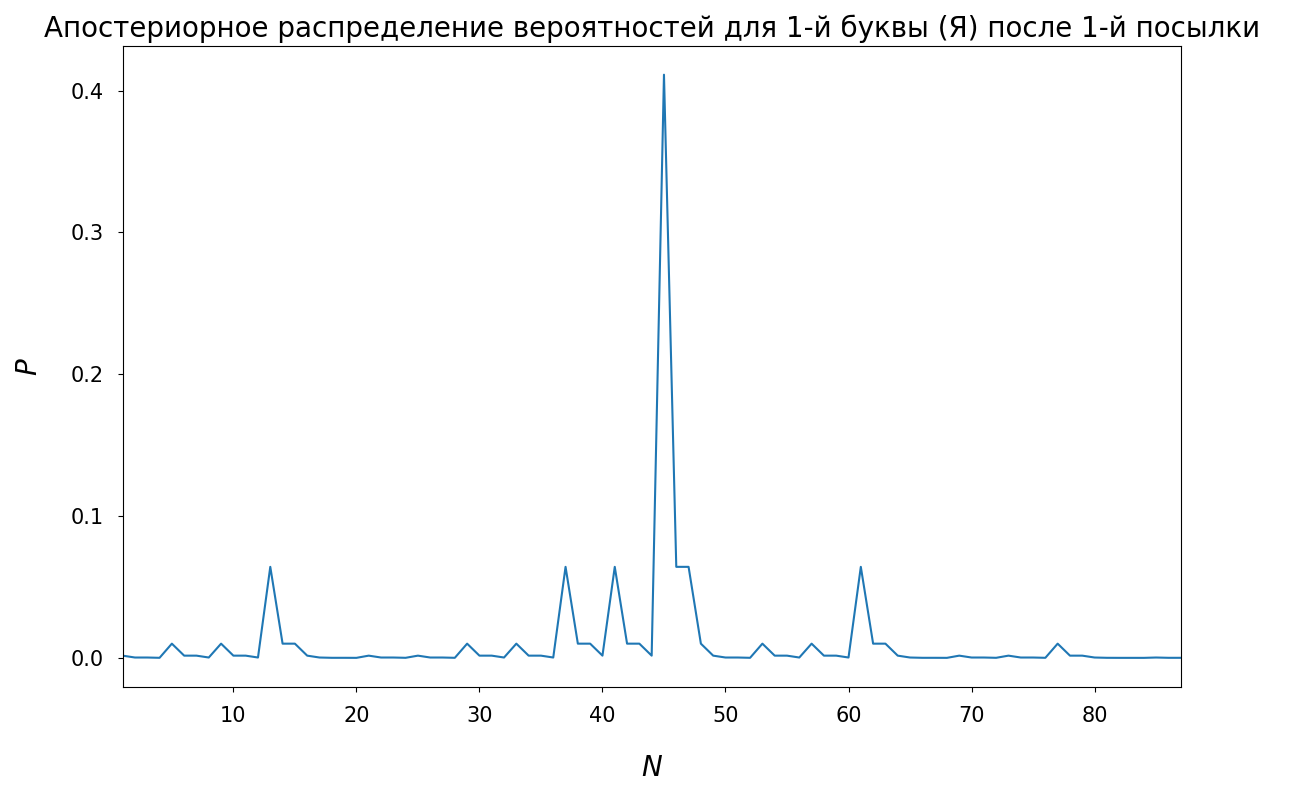
\includegraphics[scale=0.25]{seq_quir_1}
		\caption{Символы равновероятны}
	\end{subfigure}
	~
	\begin{subfigure}[b]{0.45\textwidth}
		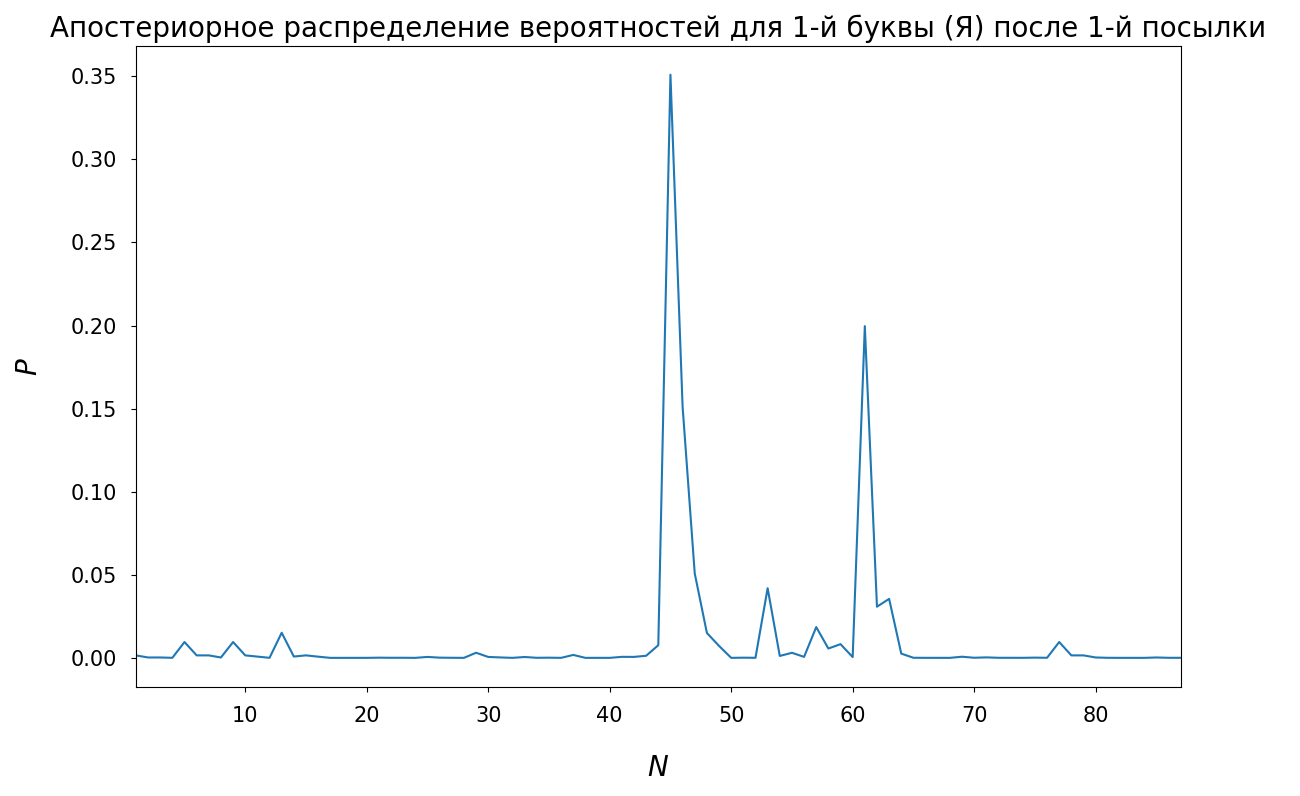
\includegraphics[scale=0.25]{seq_cyr_1}
		\caption{Вероятности согласно частотам}
	\end{subfigure}
	\caption{}
	\label{pic:3:1}
\end{center}
\end{figure}

\begin{figure}[H]
\begin{center}
	\begin{subfigure}[b]{0.45\textwidth}
		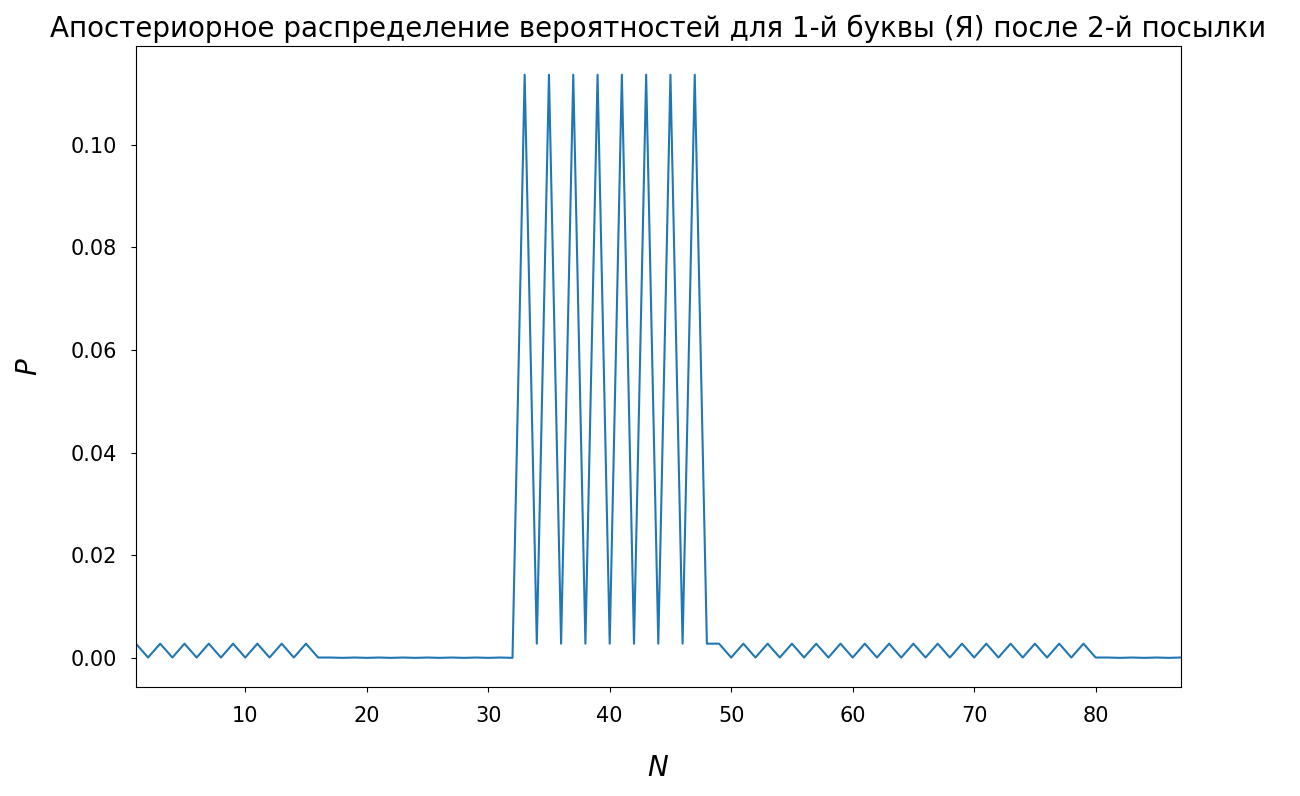
\includegraphics[scale=0.25]{seq_quir_2}
		\caption{Символы равновероятны}
	\end{subfigure}
	~
	\begin{subfigure}[b]{0.45\textwidth}
		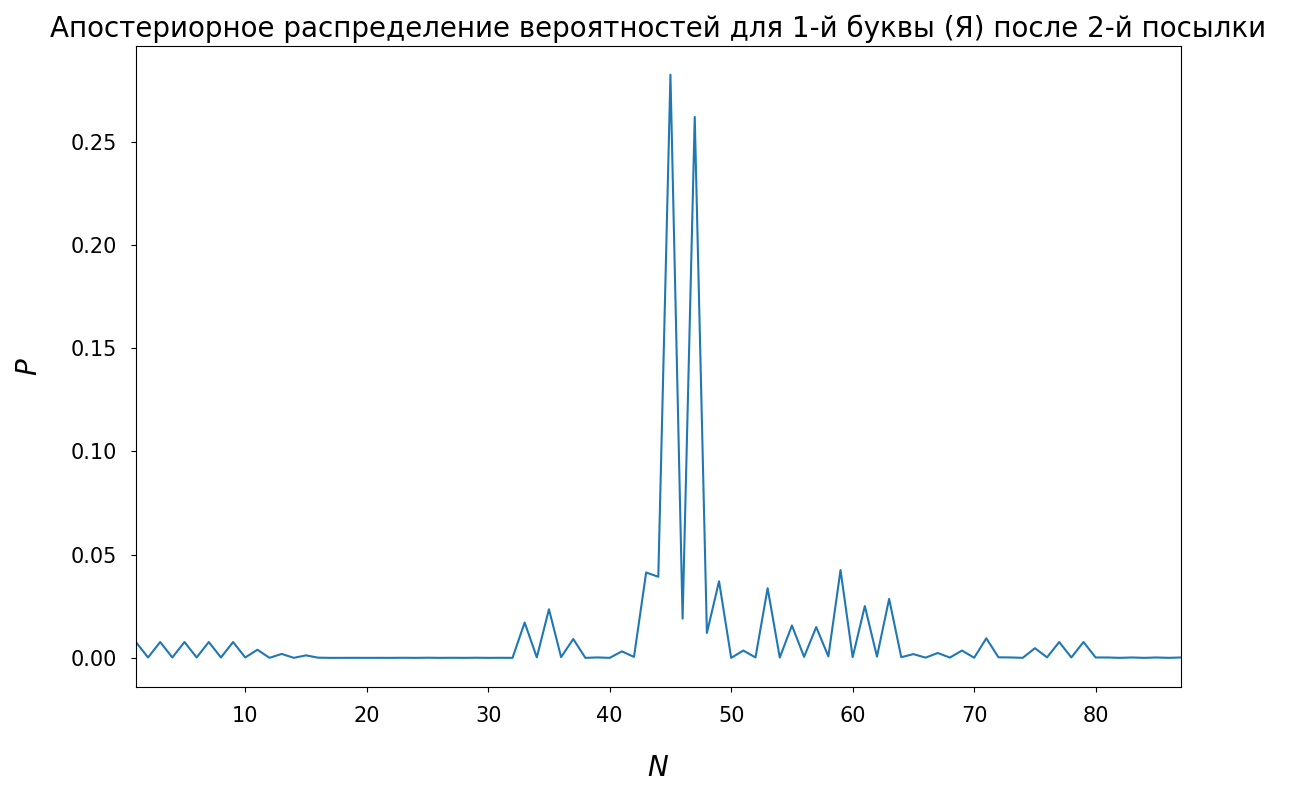
\includegraphics[scale=0.25]{seq_cyr_2}
		\caption{Вероятности согласно частотам}
	\end{subfigure}
	\caption{}
\end{center}
\end{figure}

\begin{figure}[H]
\begin{center}
	\begin{subfigure}[b]{0.45\textwidth}
		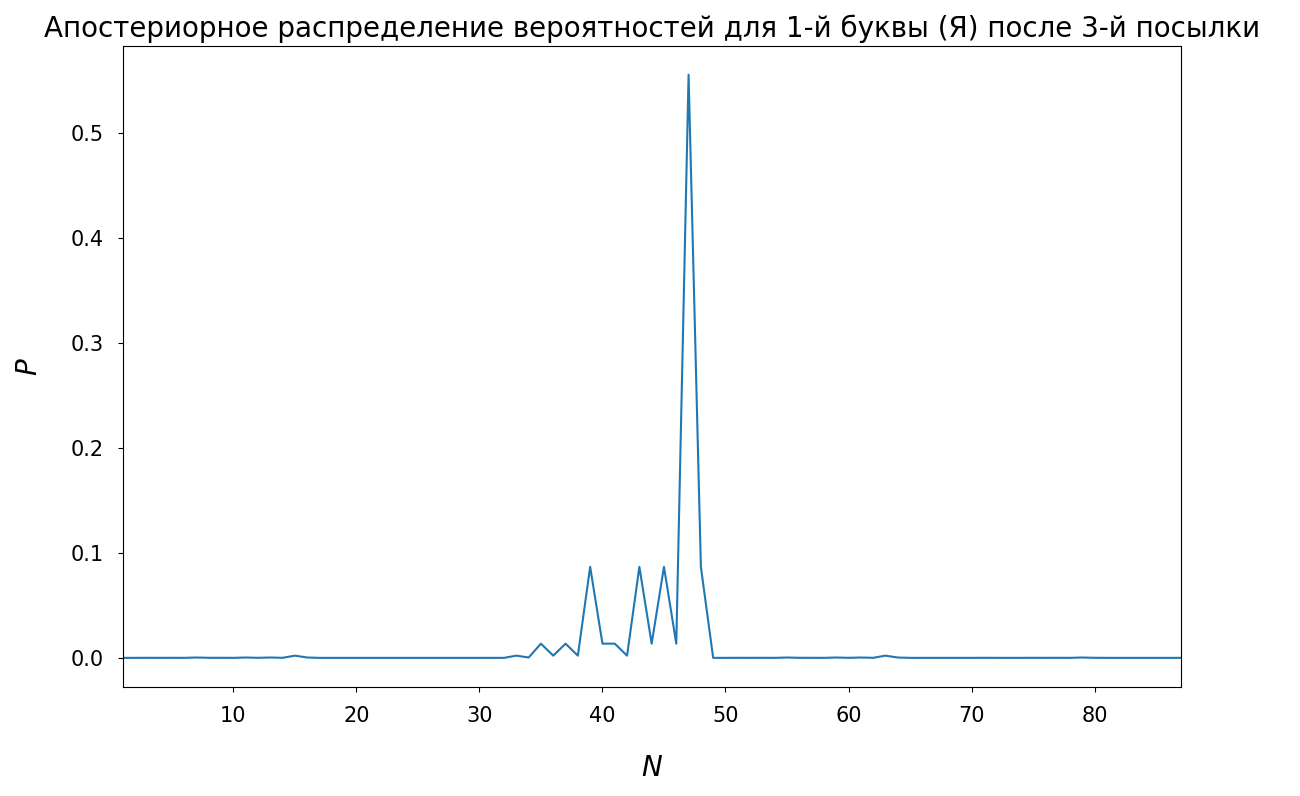
\includegraphics[scale=0.25]{seq_quir_3}
		\caption{Символы равновероятны}
	\end{subfigure}
	~
	\begin{subfigure}[b]{0.45\textwidth}
		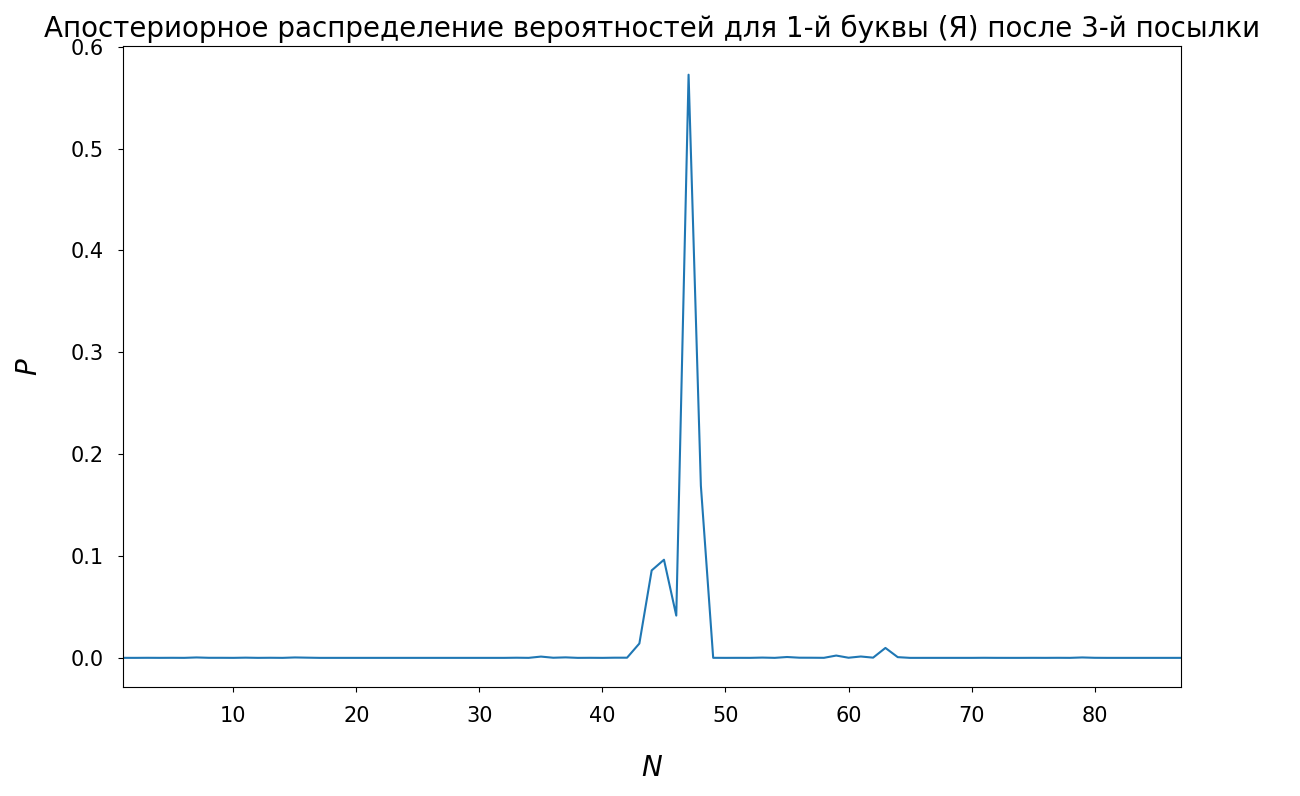
\includegraphics[scale=0.25]{seq_cyr_3}
		\caption{Вероятности согласно частотам}
	\end{subfigure}
	\caption{}
\end{center}
\end{figure}

\begin{figure}[H]
\begin{center}
	\begin{subfigure}[b]{0.45\textwidth}
		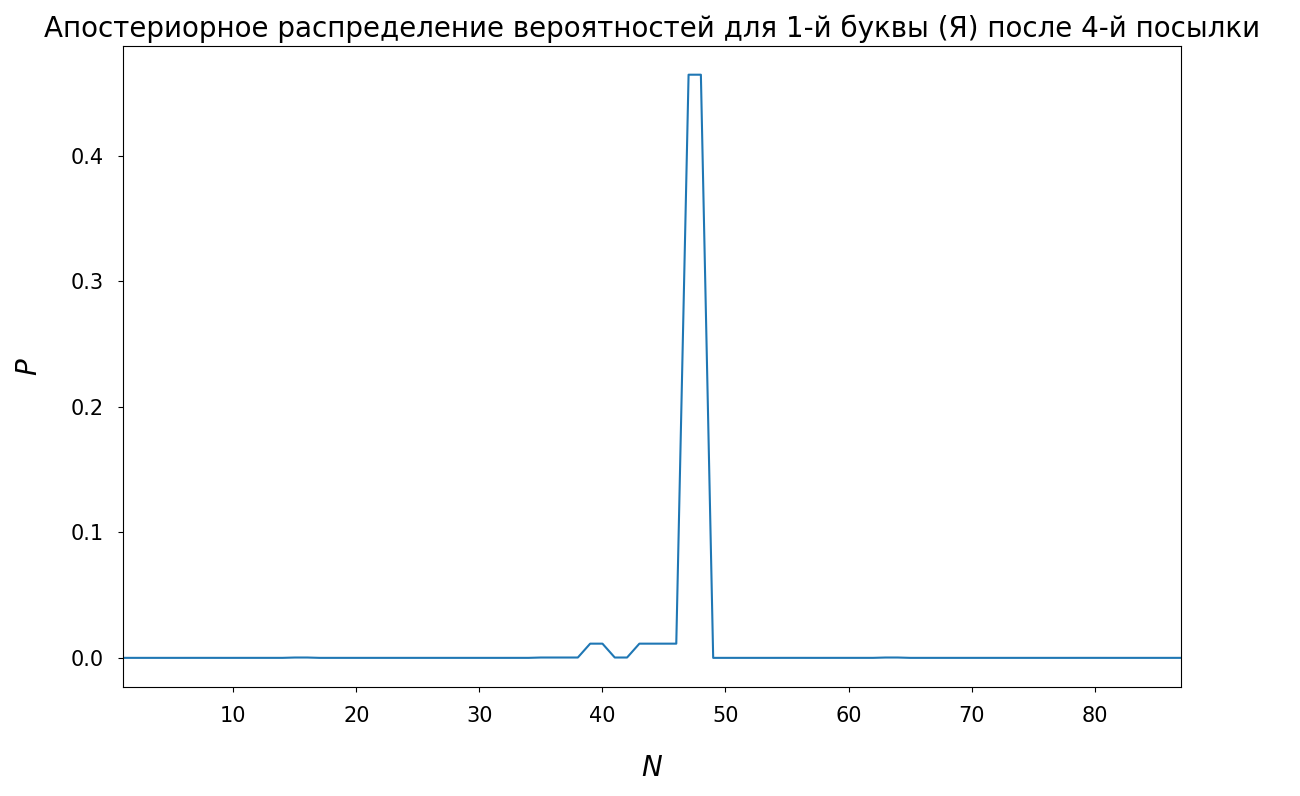
\includegraphics[scale=0.25]{seq_quir_4}
		\caption{Символы равновероятны}
	\end{subfigure}
	~
	\begin{subfigure}[b]{0.45\textwidth}
		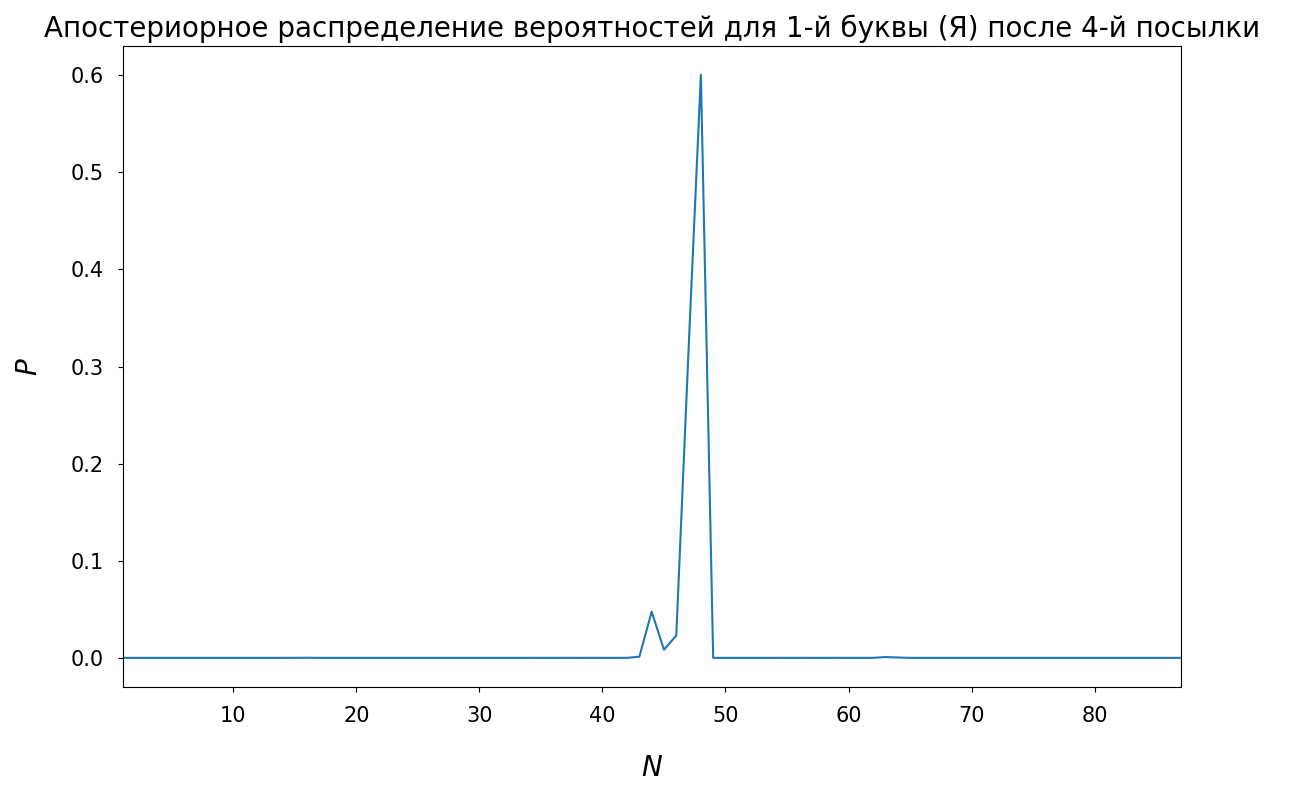
\includegraphics[scale=0.25]{seq_cyr_4}
		\caption{Вероятности согласно частотам}
	\end{subfigure}
	\caption{}
\end{center}
\end{figure}

\begin{figure}[H]
\begin{center}
	\begin{subfigure}[b]{0.45\textwidth}
		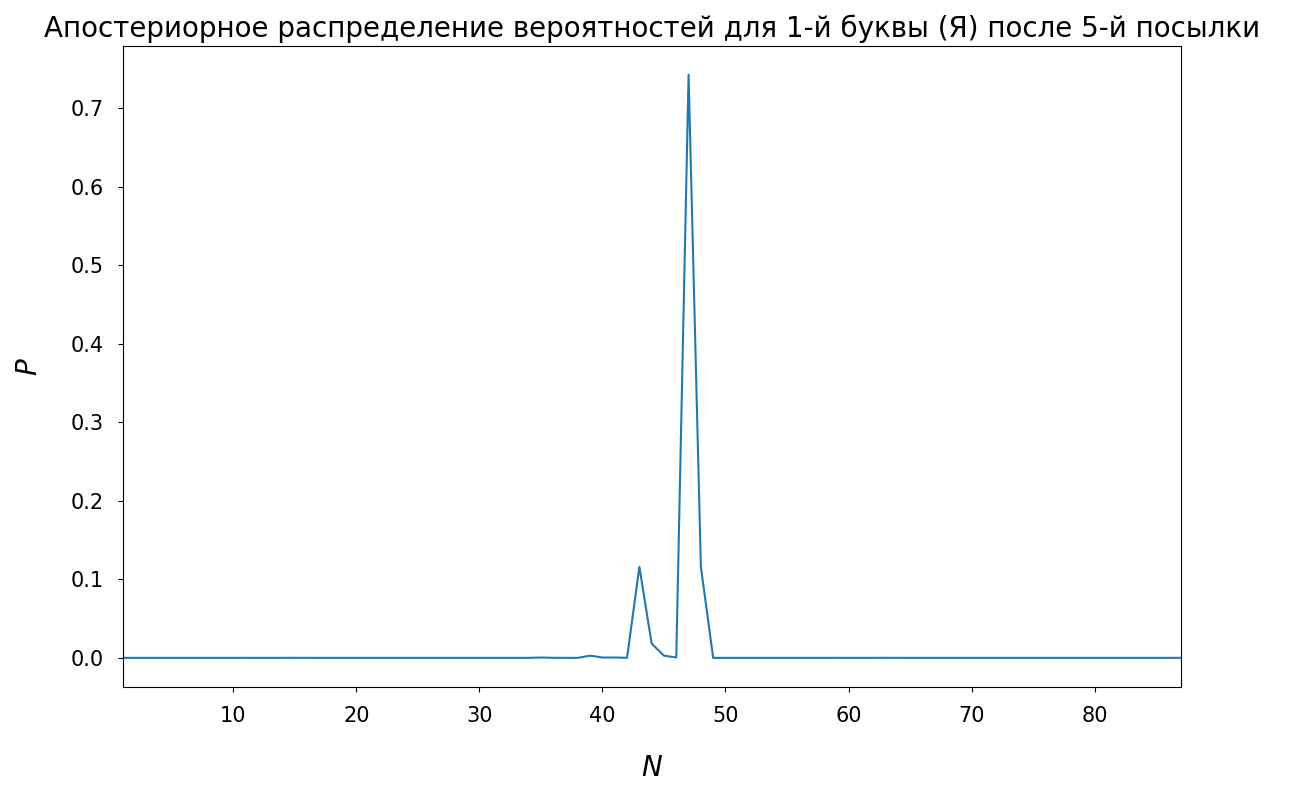
\includegraphics[scale=0.25]{seq_quir_5}
		\caption{Символы равновероятны}
	\end{subfigure}
	~
	\begin{subfigure}[b]{0.45\textwidth}
		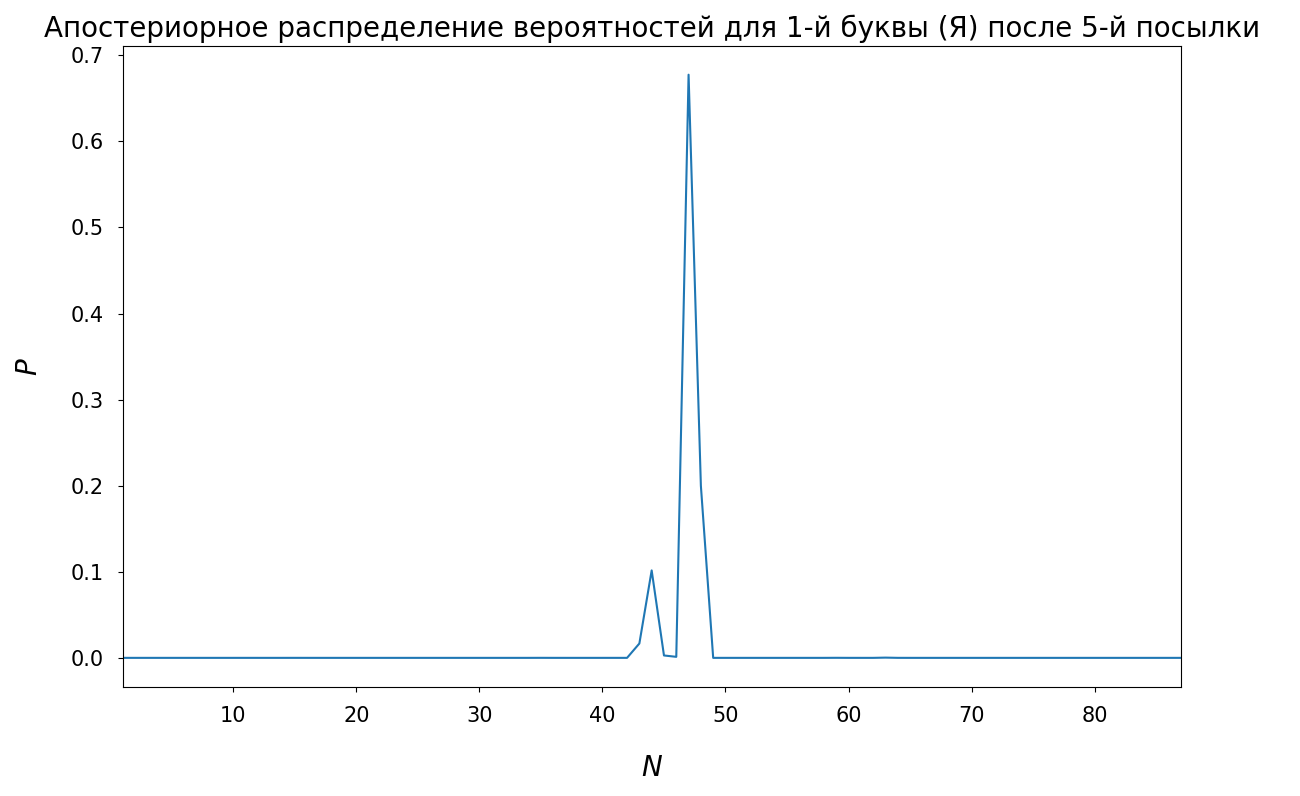
\includegraphics[scale=0.25]{seq_cyr_5}
		\caption{Вероятности согласно частотам}
	\end{subfigure}
	\caption{}
\end{center}
\end{figure}

\begin{figure}[H]
\begin{center}
	\begin{subfigure}[b]{0.45\textwidth}
		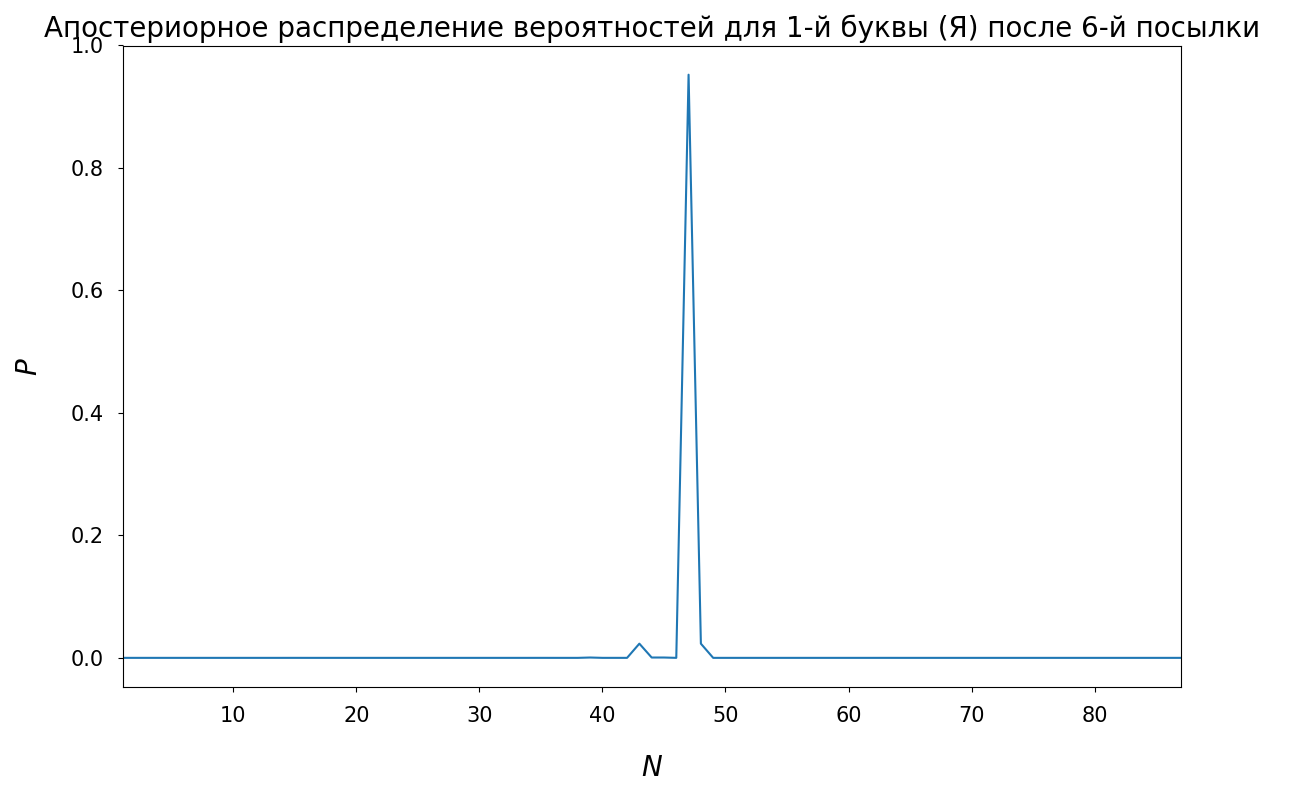
\includegraphics[scale=0.25]{seq_quir_6}
		\caption{Символы равновероятны}
	\end{subfigure}
	~
	\begin{subfigure}[b]{0.45\textwidth}
		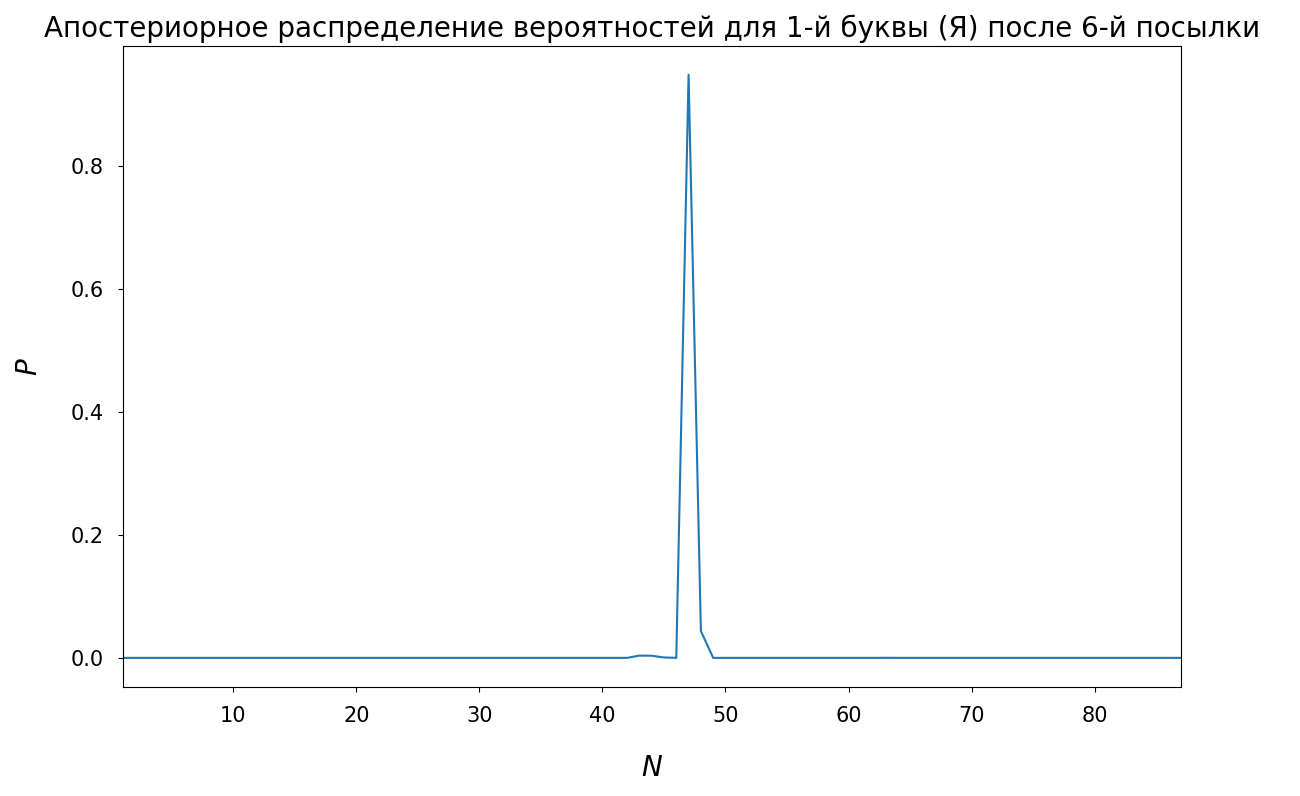
\includegraphics[scale=0.25]{seq_cyr_6}
		\caption{Вероятности согласно частотам}
	\end{subfigure}
	\caption{}
\end{center}
\end{figure}

\begin{figure}[H]
\begin{center}
	\begin{subfigure}[b]{0.45\textwidth}
		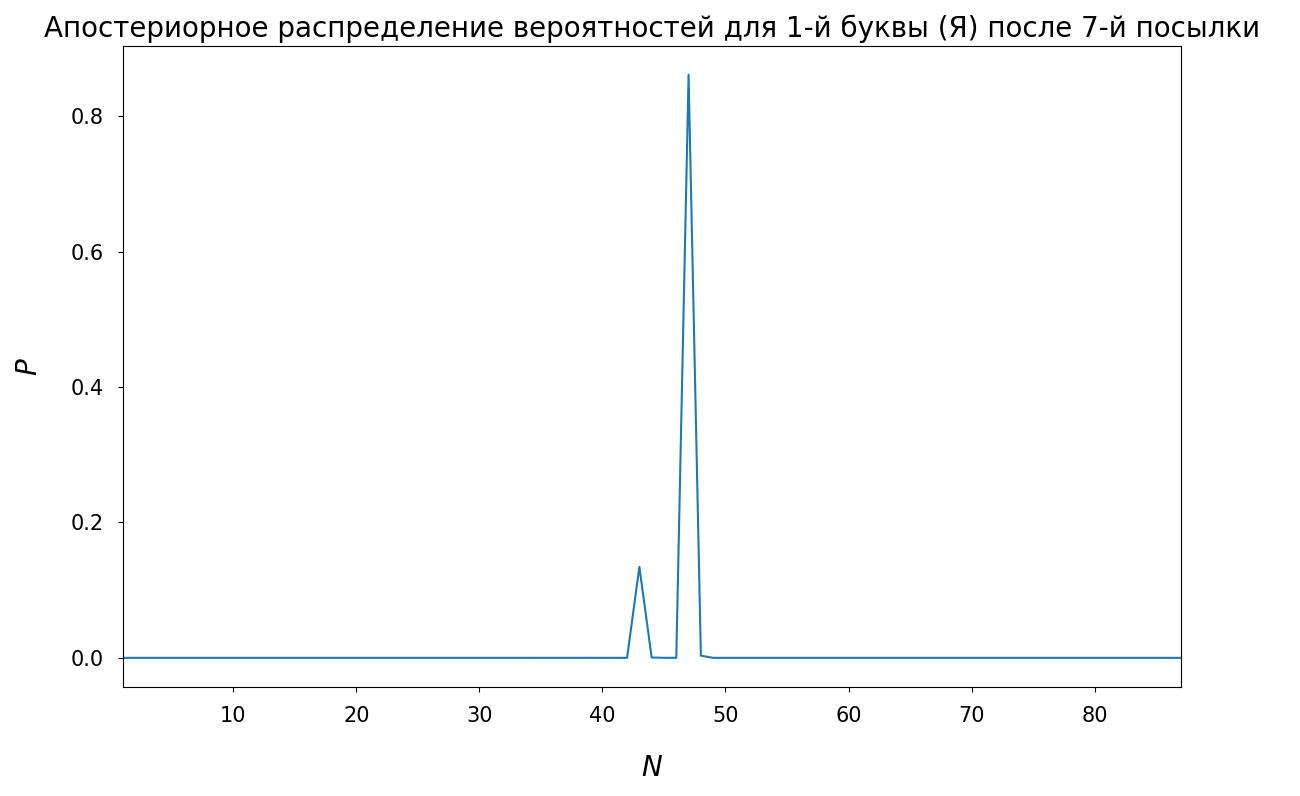
\includegraphics[scale=0.25]{seq_quir_7}
		\caption{Символы равновероятны}
	\end{subfigure}
	~
	\begin{subfigure}[b]{0.45\textwidth}
		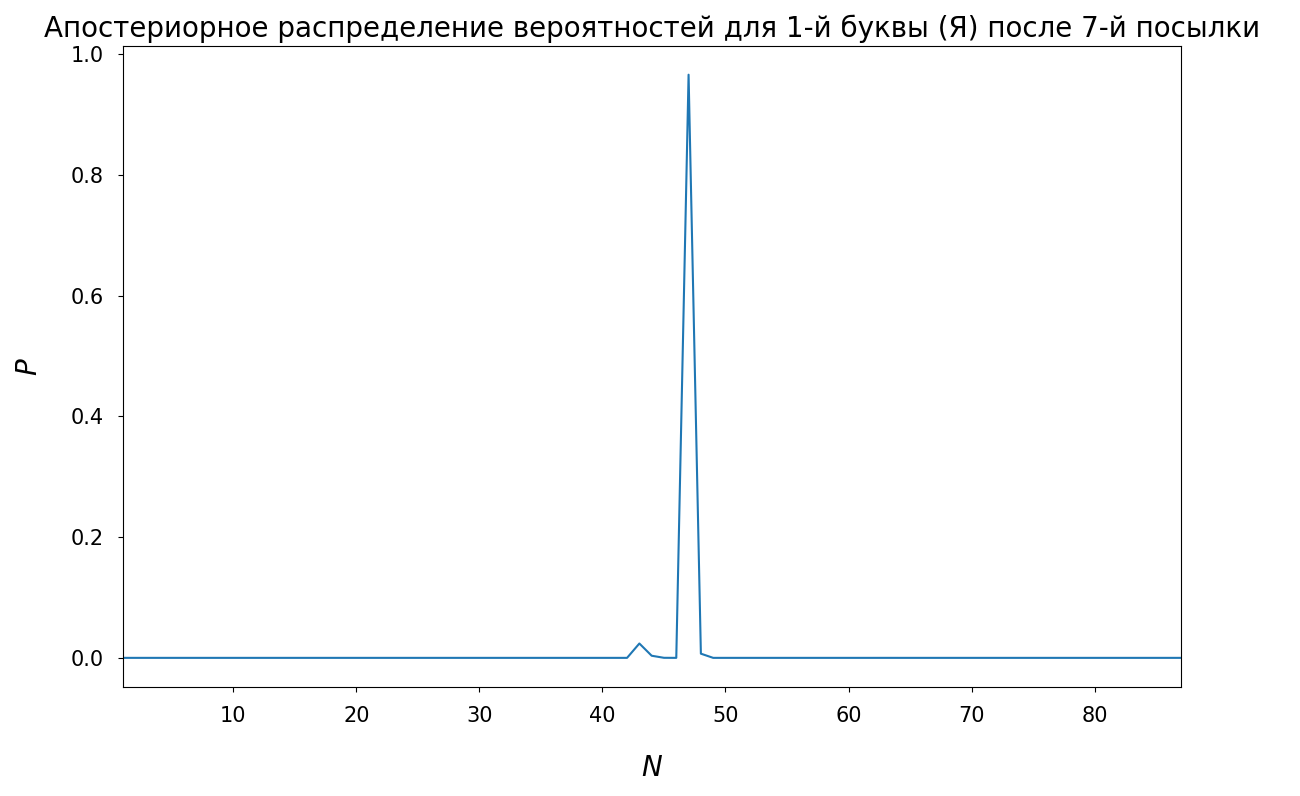
\includegraphics[scale=0.25]{seq_cyr_7}
		\caption{Вероятности согласно частотам}
	\end{subfigure}
	\caption{}
\end{center}
\end{figure}

\begin{figure}[H]
\begin{center}
	\begin{subfigure}[b]{0.45\textwidth}
		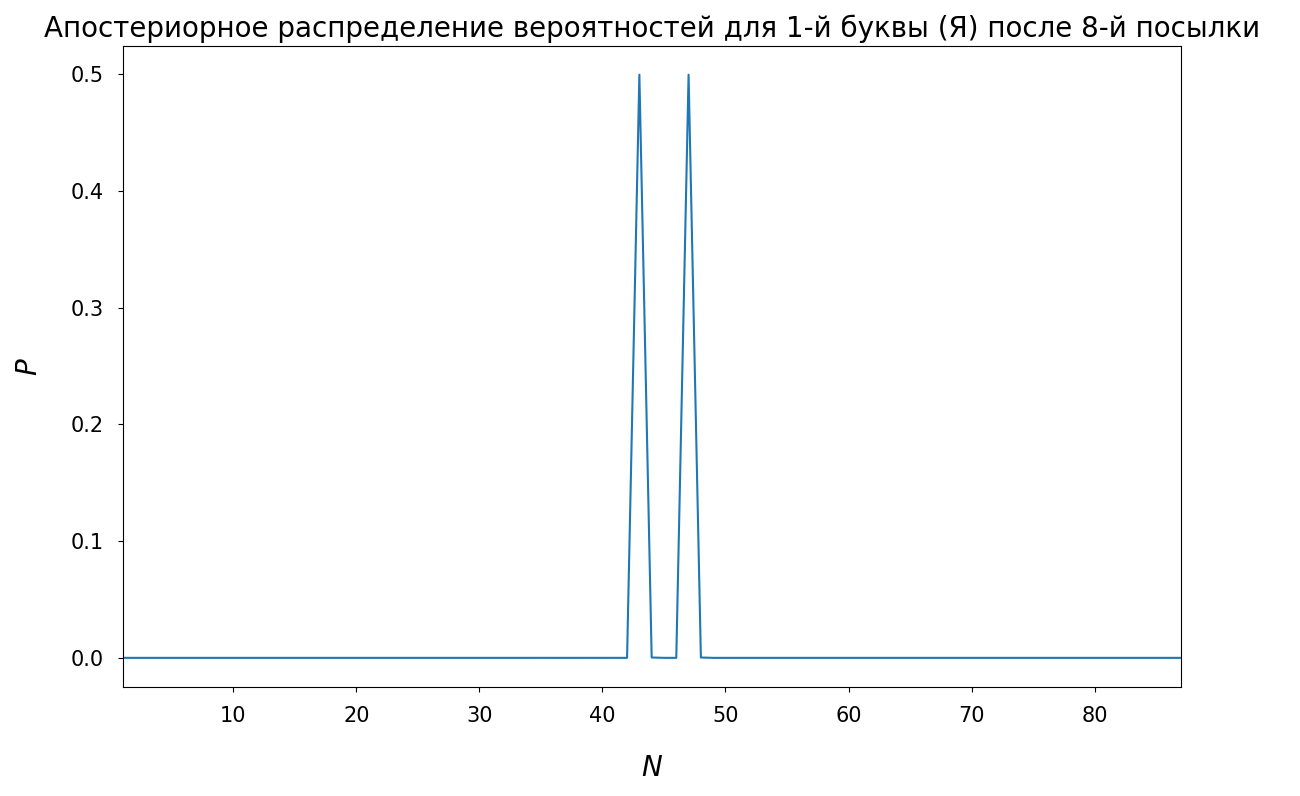
\includegraphics[scale=0.25]{seq_quir_8}
		\caption{Символы равновероятны}
	\end{subfigure}
	~
	\begin{subfigure}[b]{0.45\textwidth}
		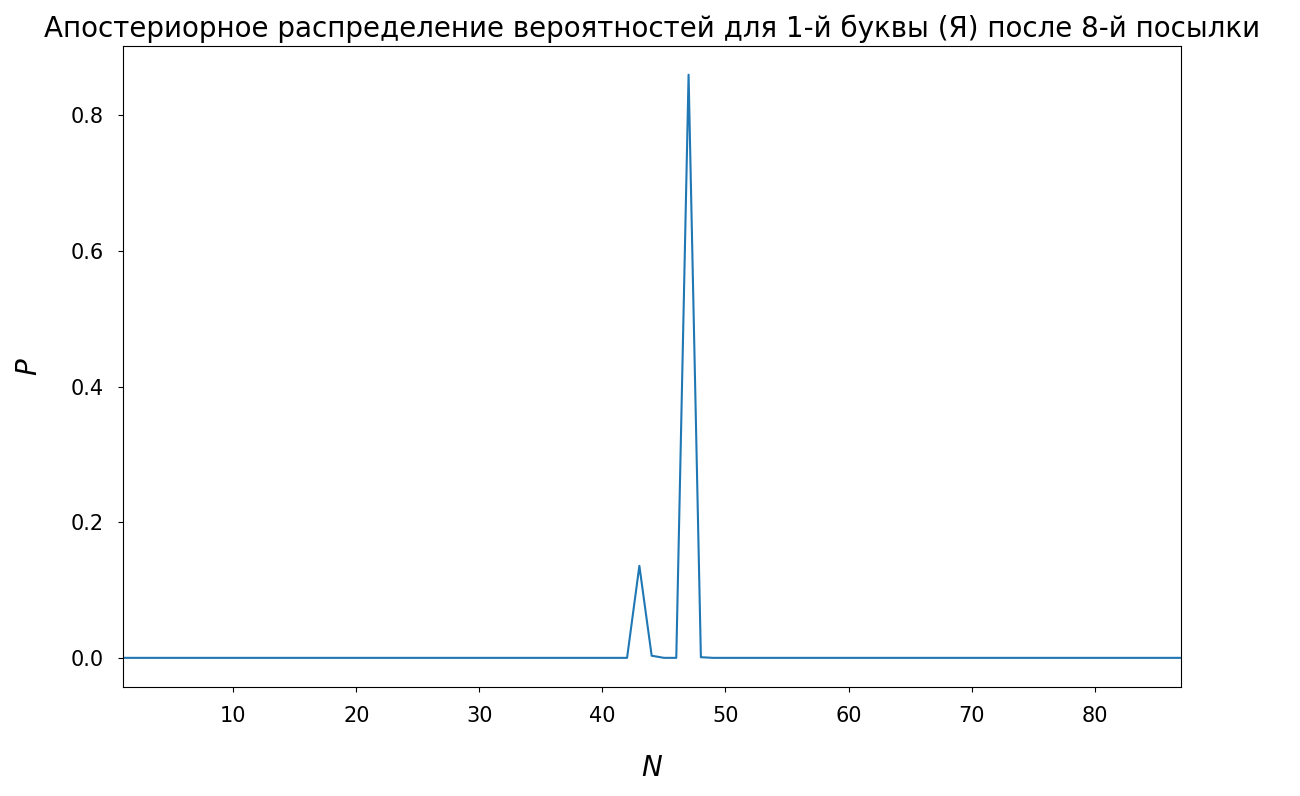
\includegraphics[scale=0.25]{seq_cyr_8}
		\caption{Вероятности согласно частотам}
	\end{subfigure}
	\caption{}
\end{center}
\end{figure}

\begin{figure}[H]
\begin{center}
	\begin{subfigure}[b]{0.45\textwidth}
		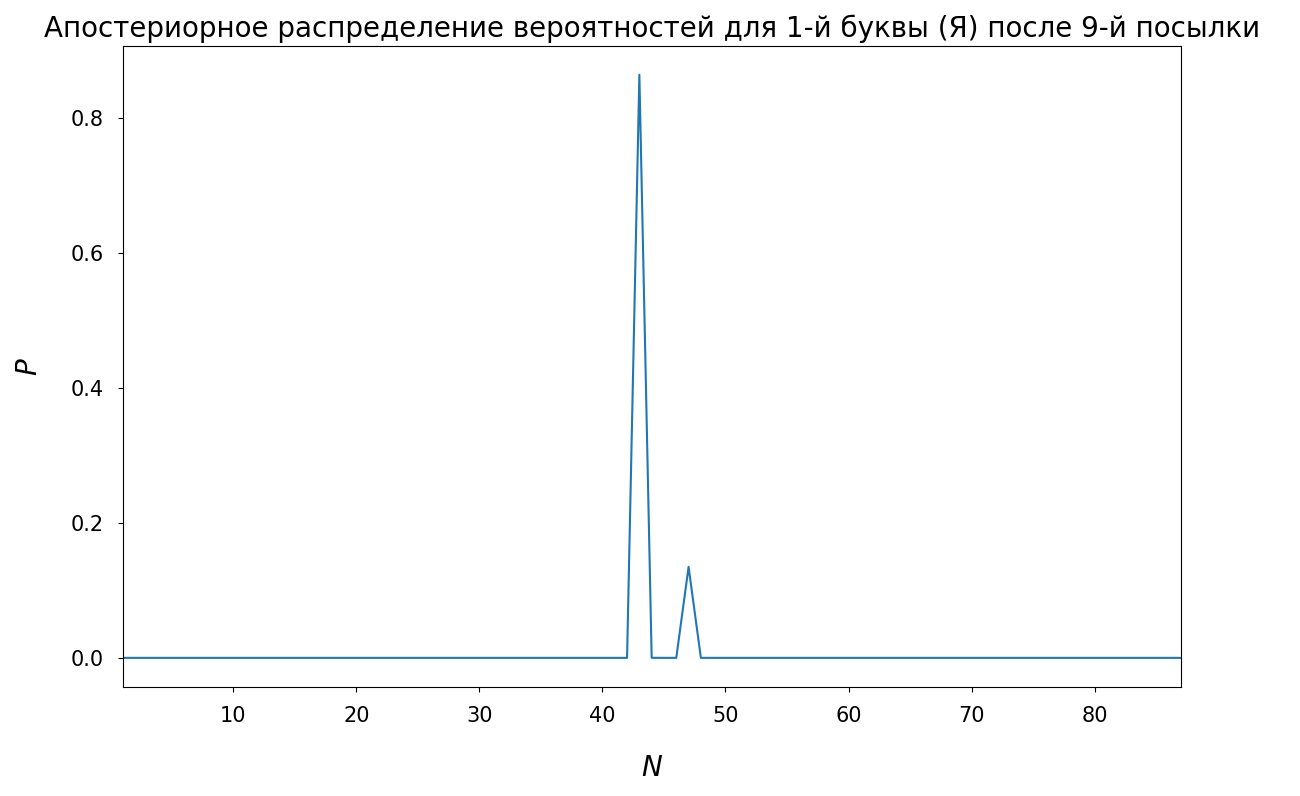
\includegraphics[scale=0.25]{seq_quir_9}
		\caption{Символы равновероятны}
	\end{subfigure}
	~
	\begin{subfigure}[b]{0.45\textwidth}
		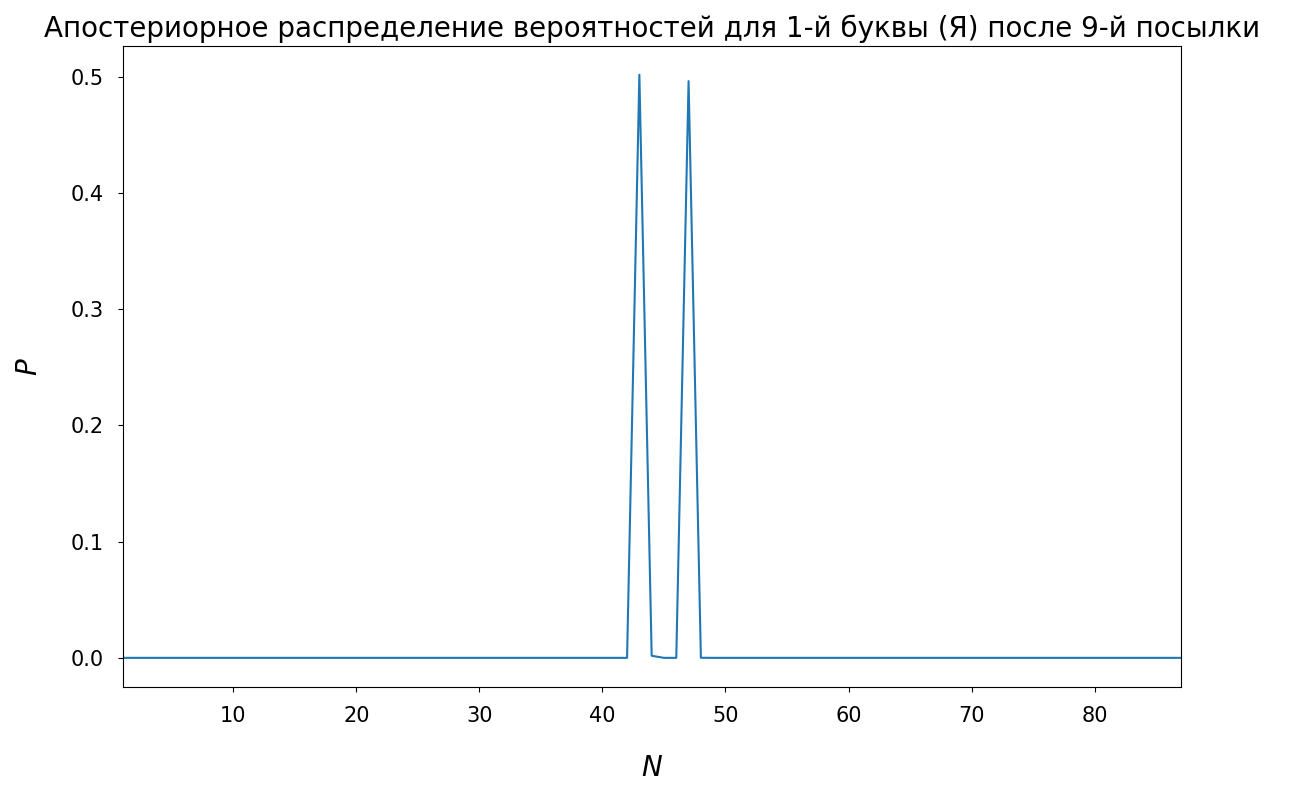
\includegraphics[scale=0.25]{seq_cyr_9}
		\caption{Вероятности согласно частотам}
	\end{subfigure}
	\caption{}
\end{center}
\end{figure}

\begin{figure}[H]
\begin{center}
	\begin{subfigure}[b]{0.45\textwidth}
		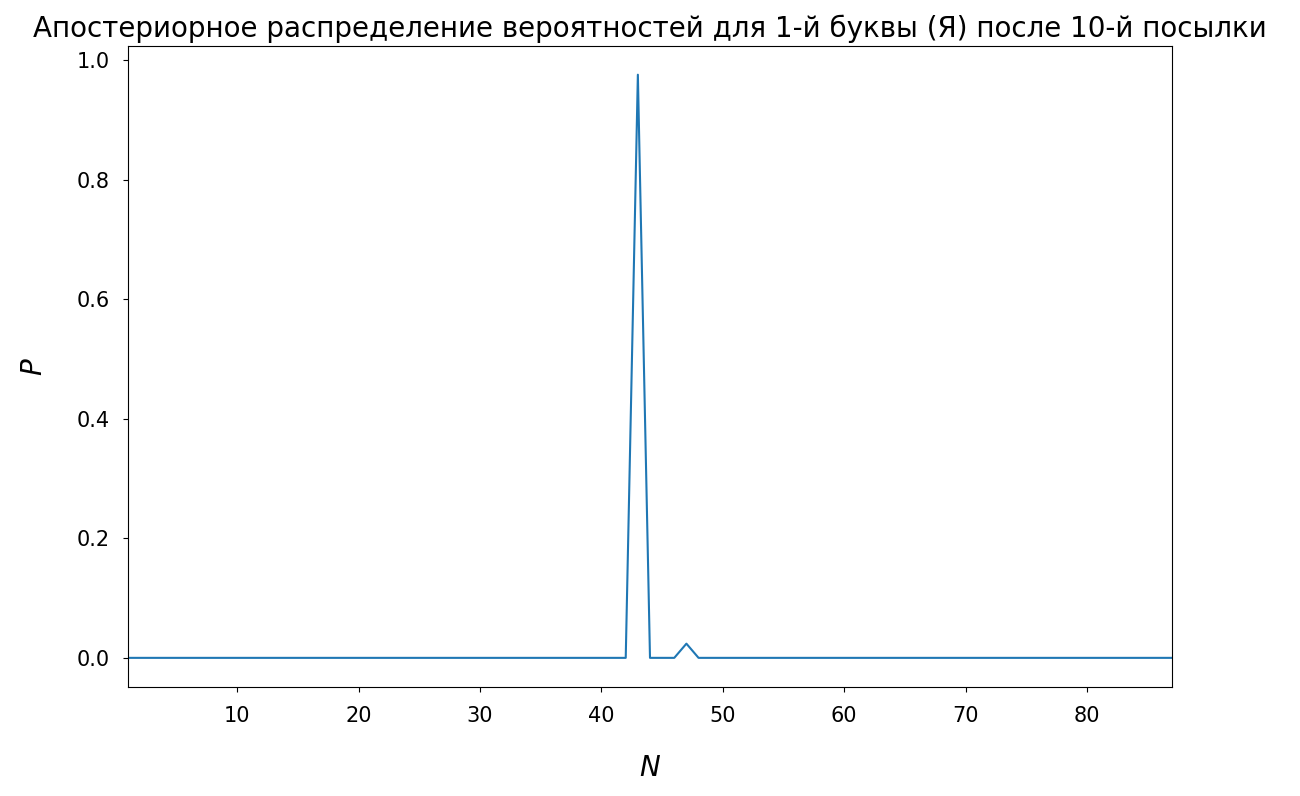
\includegraphics[scale=0.25]{seq_quir_10}
		\caption{Символы равновероятны}
	\end{subfigure}
	~
	\begin{subfigure}[b]{0.45\textwidth}
		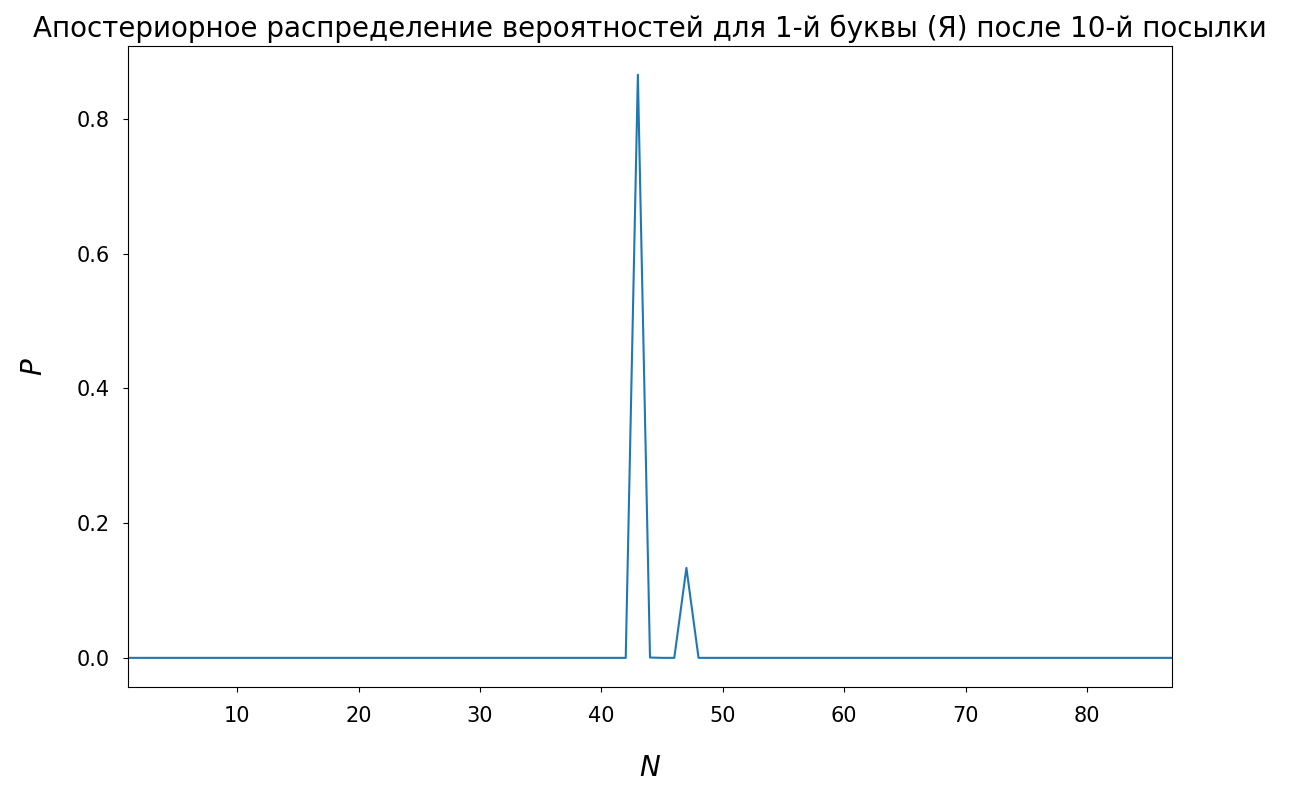
\includegraphics[scale=0.25]{seq_cyr_10}
		\caption{Вероятности согласно частотам}
	\end{subfigure}
	\caption{}
\end{center}
\end{figure}

\begin{figure}[H]
\begin{center}
	\begin{subfigure}[b]{0.45\textwidth}
		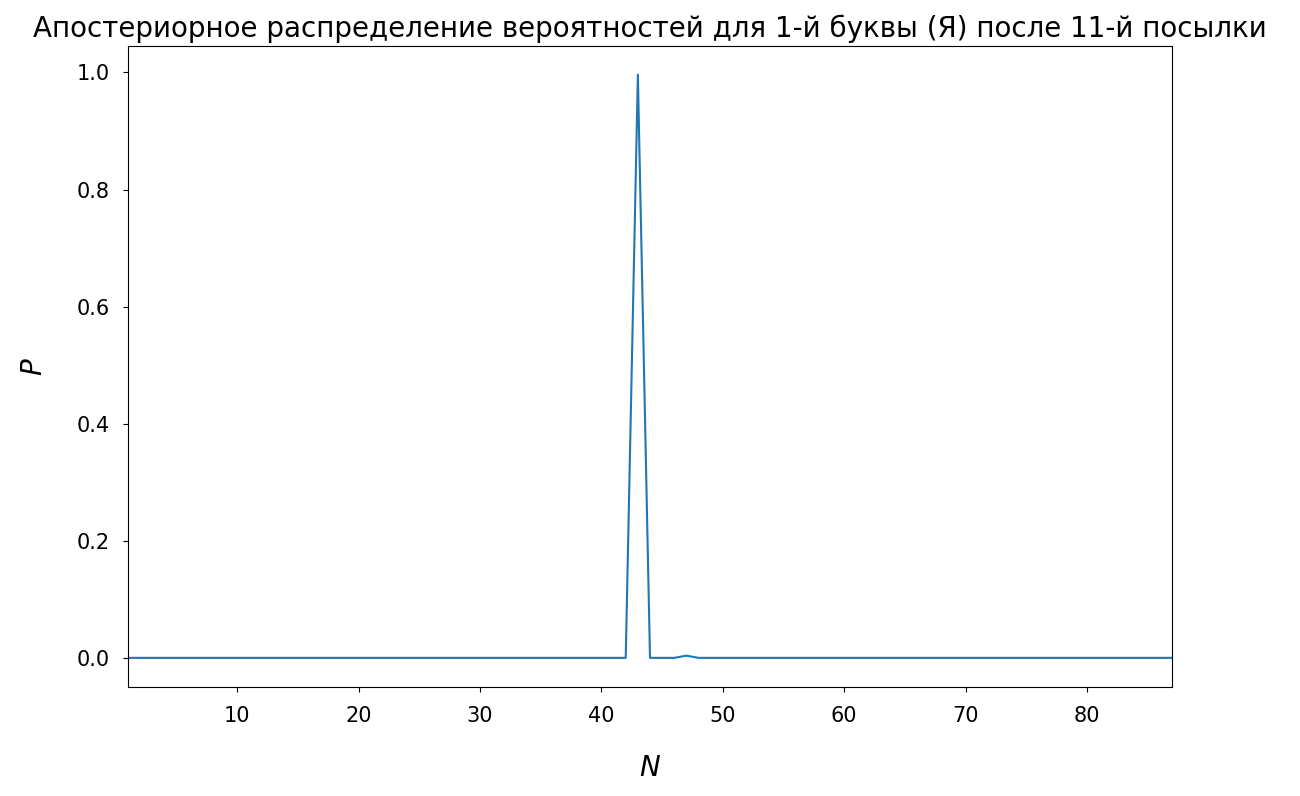
\includegraphics[scale=0.25]{seq_quir_11}
		\caption{Символы равновероятны}
	\end{subfigure}
	~
	\begin{subfigure}[b]{0.45\textwidth}
		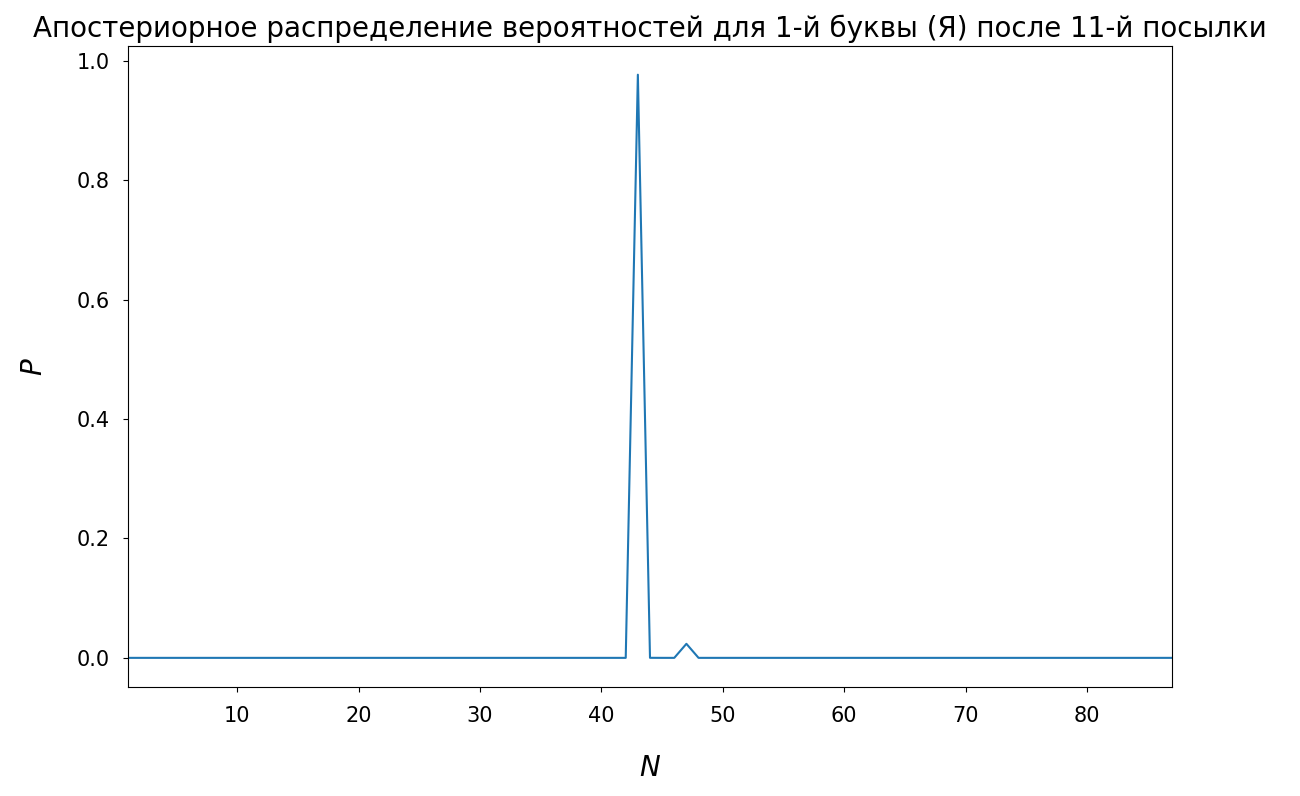
\includegraphics[scale=0.25]{seq_cyr_11}
		\caption{Вероятности согласно частотам}
	\end{subfigure}
	\caption{}
\end{center}
\end{figure}

\begin{figure}[H]
\begin{center}
	\begin{subfigure}[b]{0.45\textwidth}
		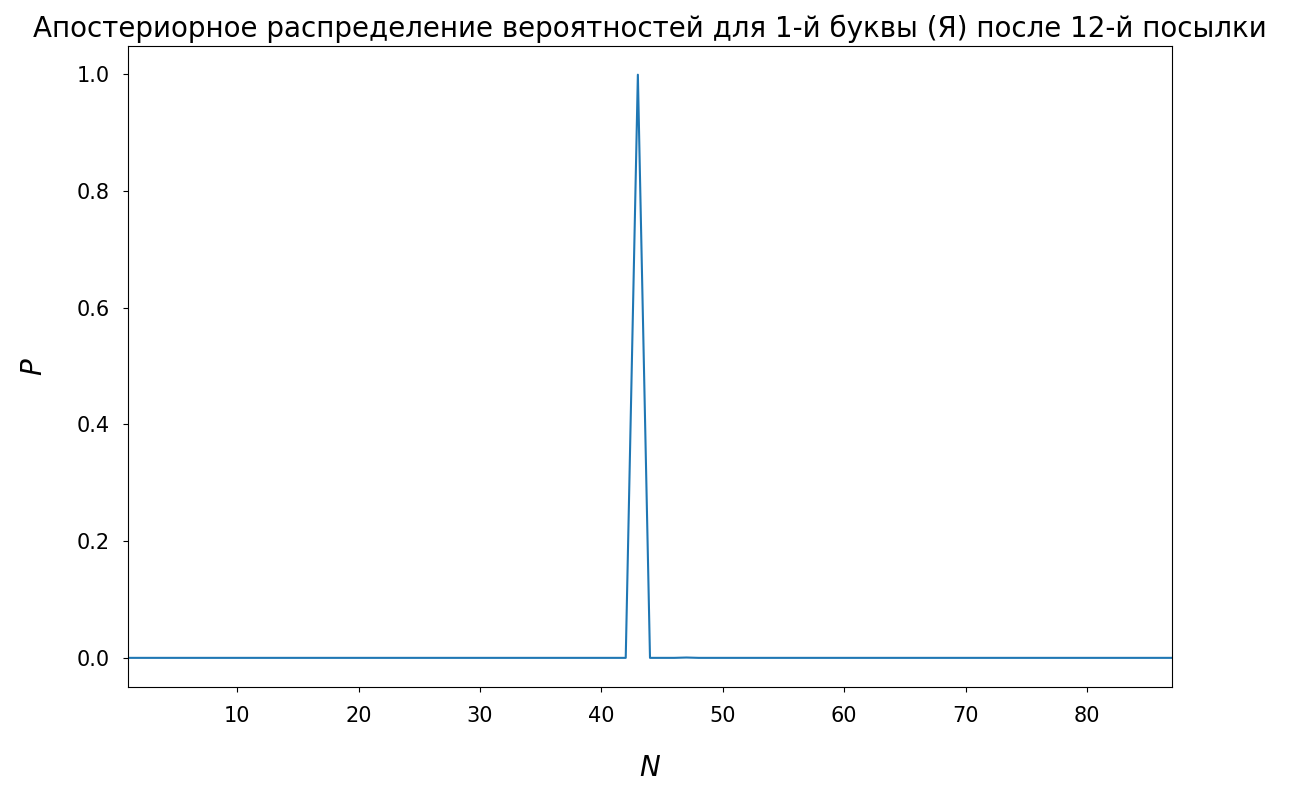
\includegraphics[scale=0.25]{seq_quir_12}
		\caption{Символы равновероятны}
	\end{subfigure}
	~
	\begin{subfigure}[b]{0.45\textwidth}
		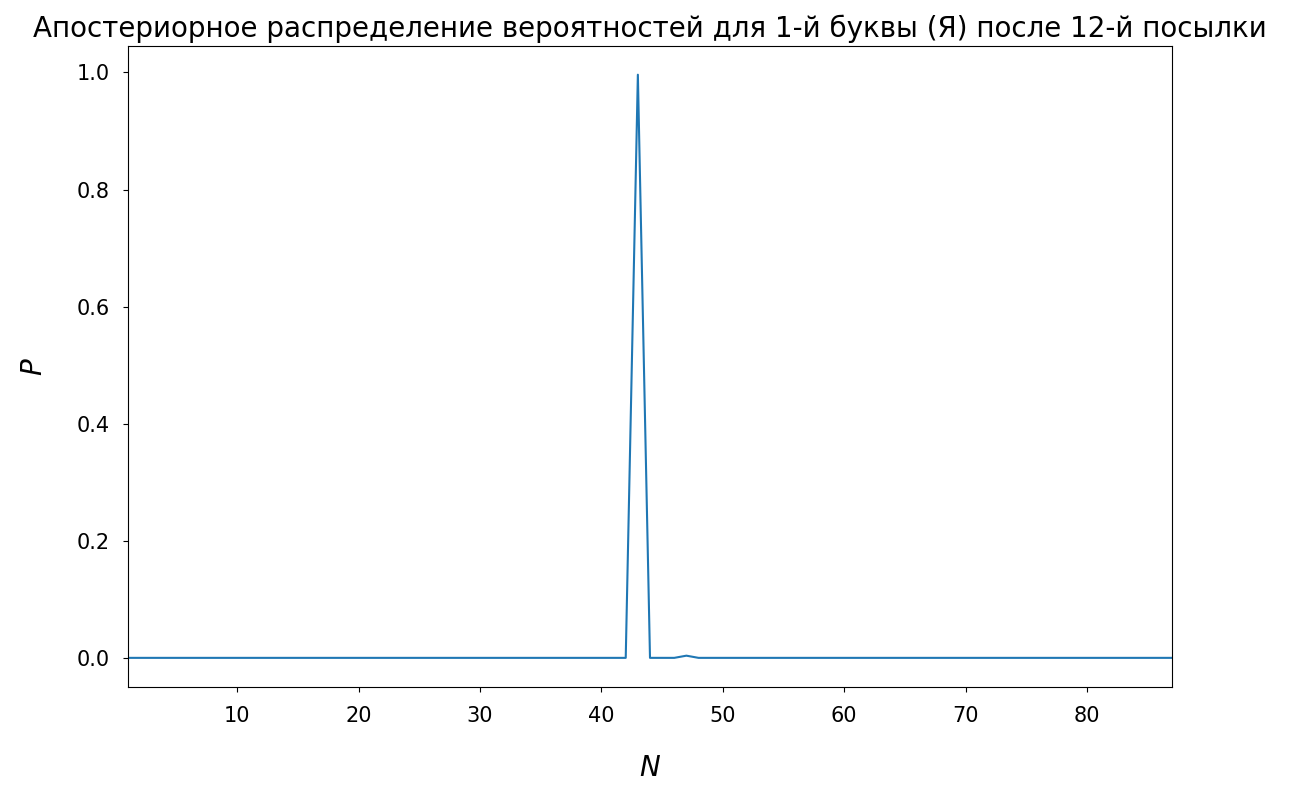
\includegraphics[scale=0.25]{seq_cyr_12}
		\caption{Вероятности согласно частотам}
	\end{subfigure}
	\caption{}
\end{center}
\end{figure}

\begin{figure}[H]
\begin{center}
	\begin{subfigure}[b]{0.45\textwidth}
		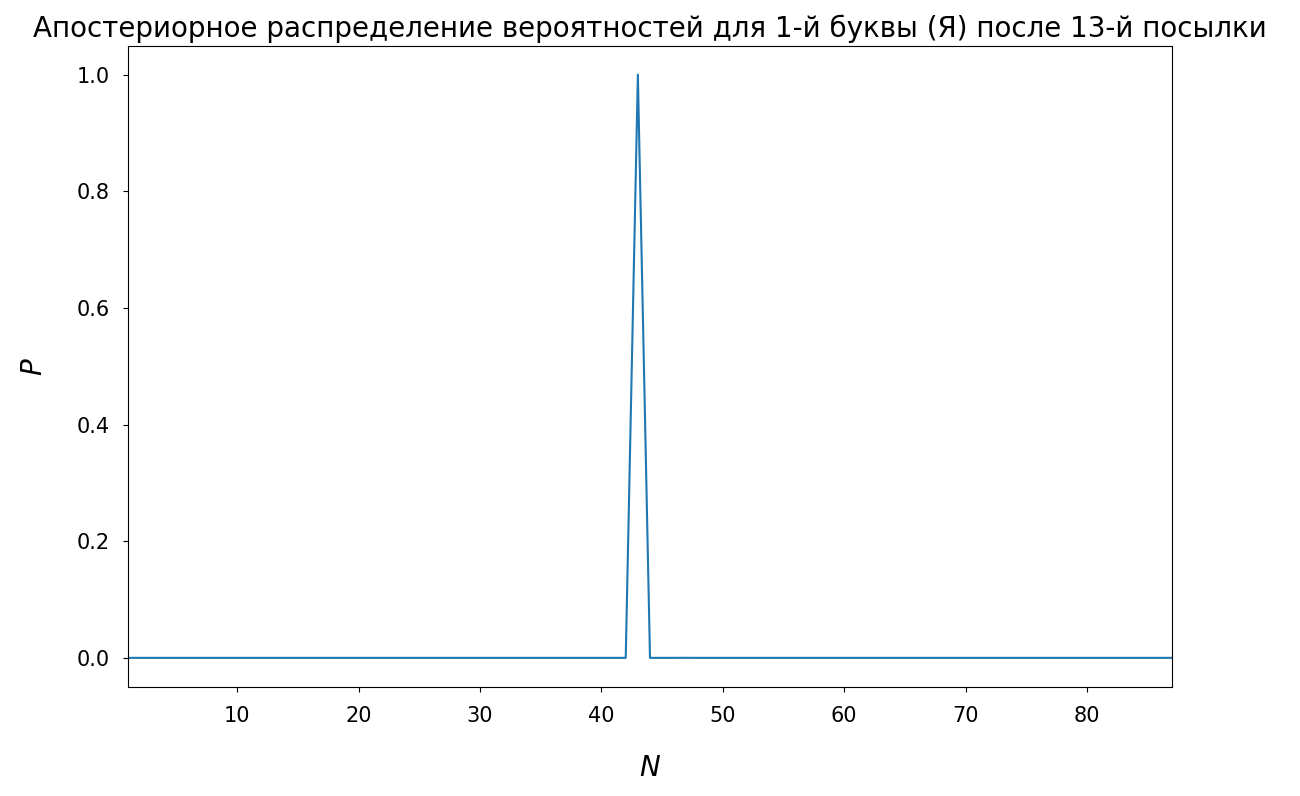
\includegraphics[scale=0.25]{seq_quir_13}
		\caption{Символы равновероятны}
	\end{subfigure}
	~
	\begin{subfigure}[b]{0.45\textwidth}
		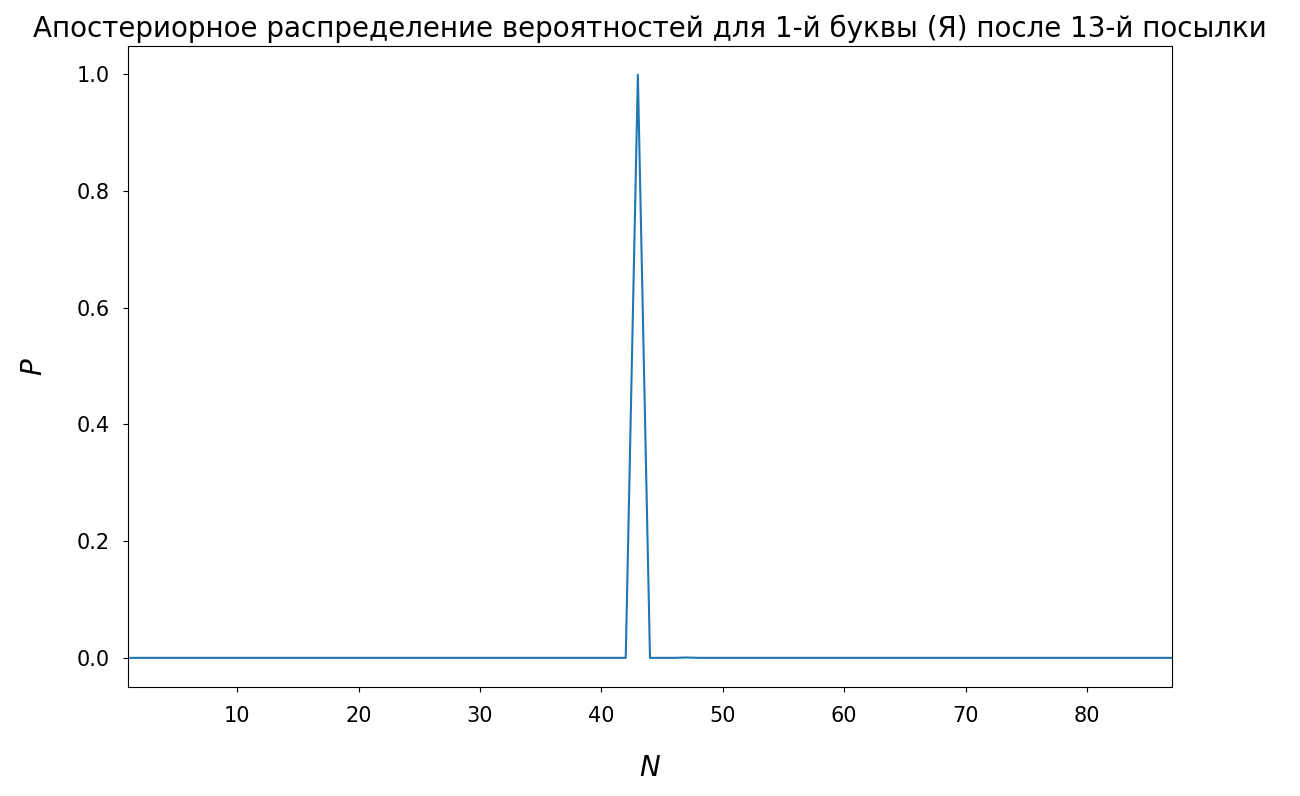
\includegraphics[scale=0.25]{seq_cyr_13}
		\caption{Вероятности согласно частотам}
	\end{subfigure}
	\caption{}
\end{center}
\end{figure}

\begin{figure}[H]
\begin{center}
	\begin{subfigure}[b]{0.45\textwidth}
		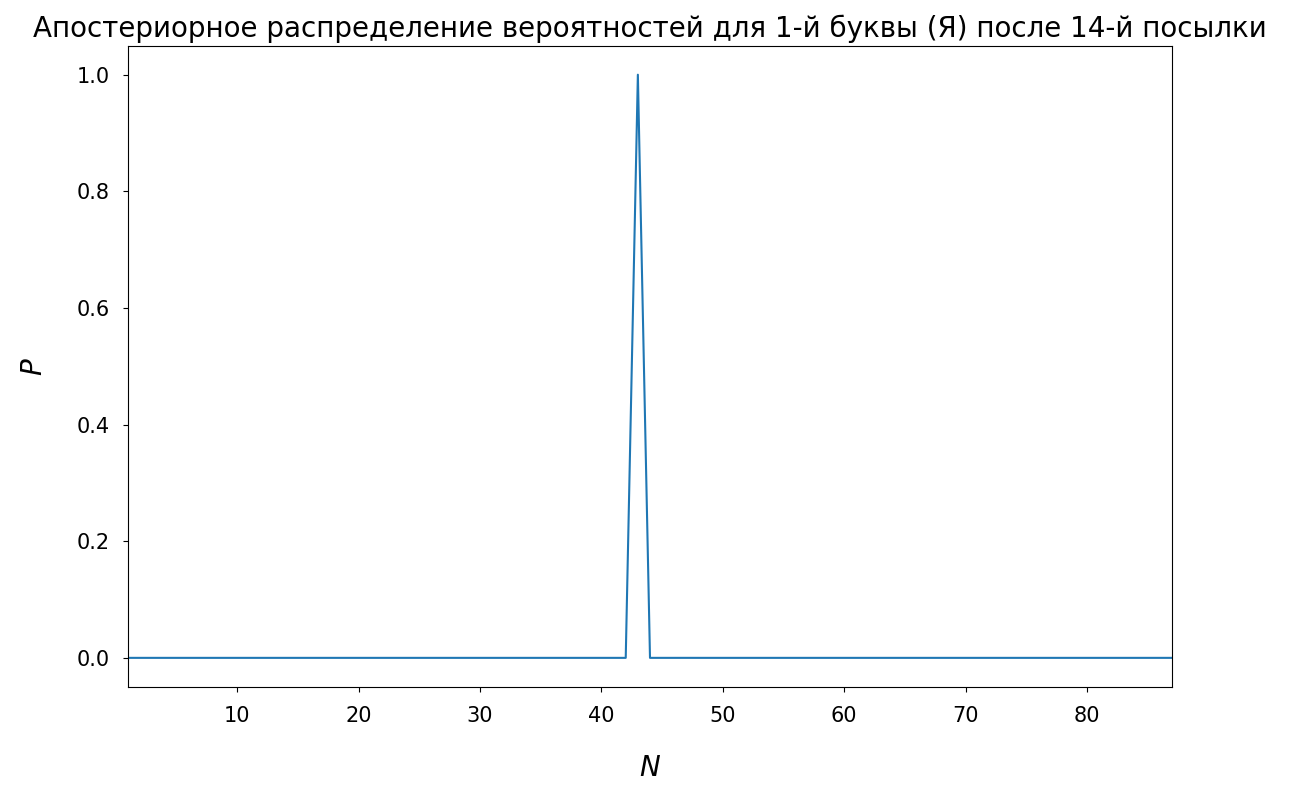
\includegraphics[scale=0.25]{seq_quir_14}
		\caption{Символы равновероятны}
	\end{subfigure}
	~
	\begin{subfigure}[b]{0.45\textwidth}
		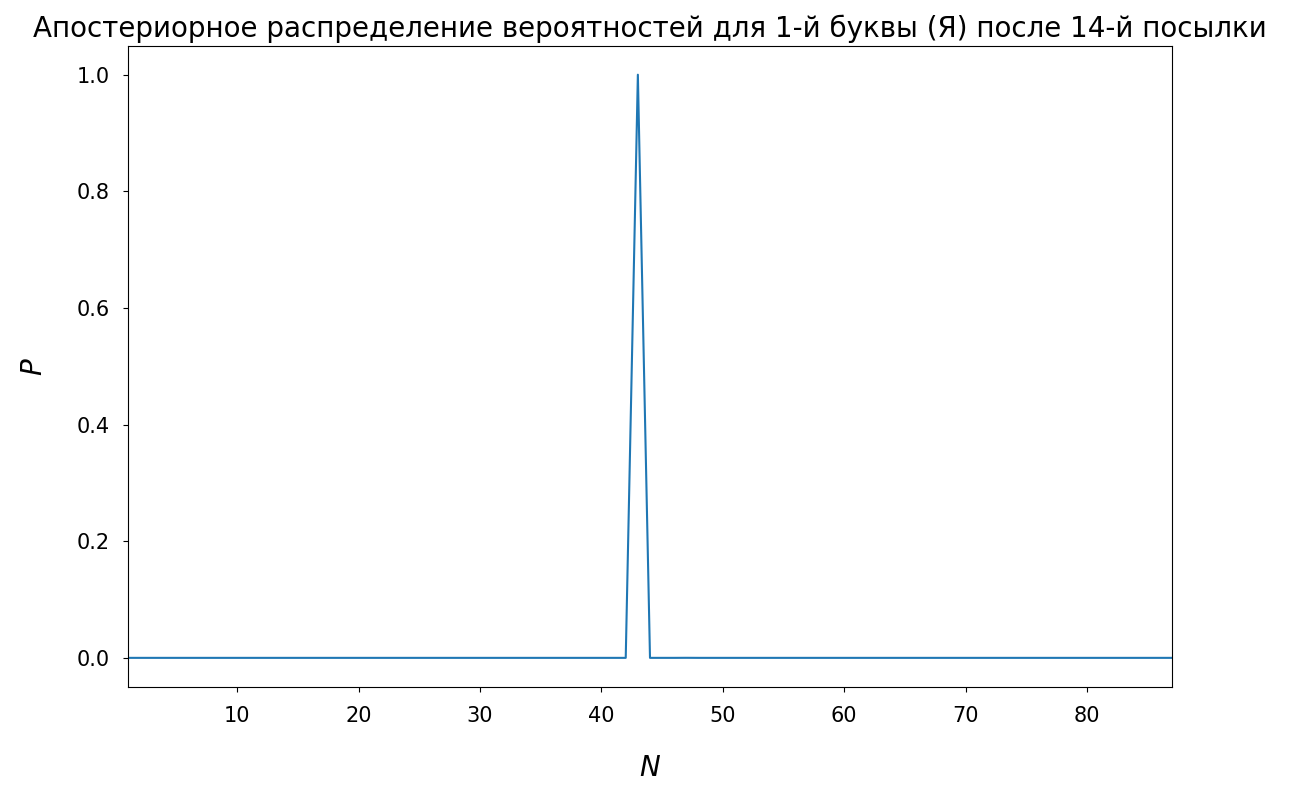
\includegraphics[scale=0.25]{seq_cyr_14}
		\caption{Вероятности согласно частотам}
	\end{subfigure}
	\caption{}
\end{center}
\end{figure}

\begin{figure}[H]
\begin{center}
	\begin{subfigure}[b]{0.45\textwidth}
		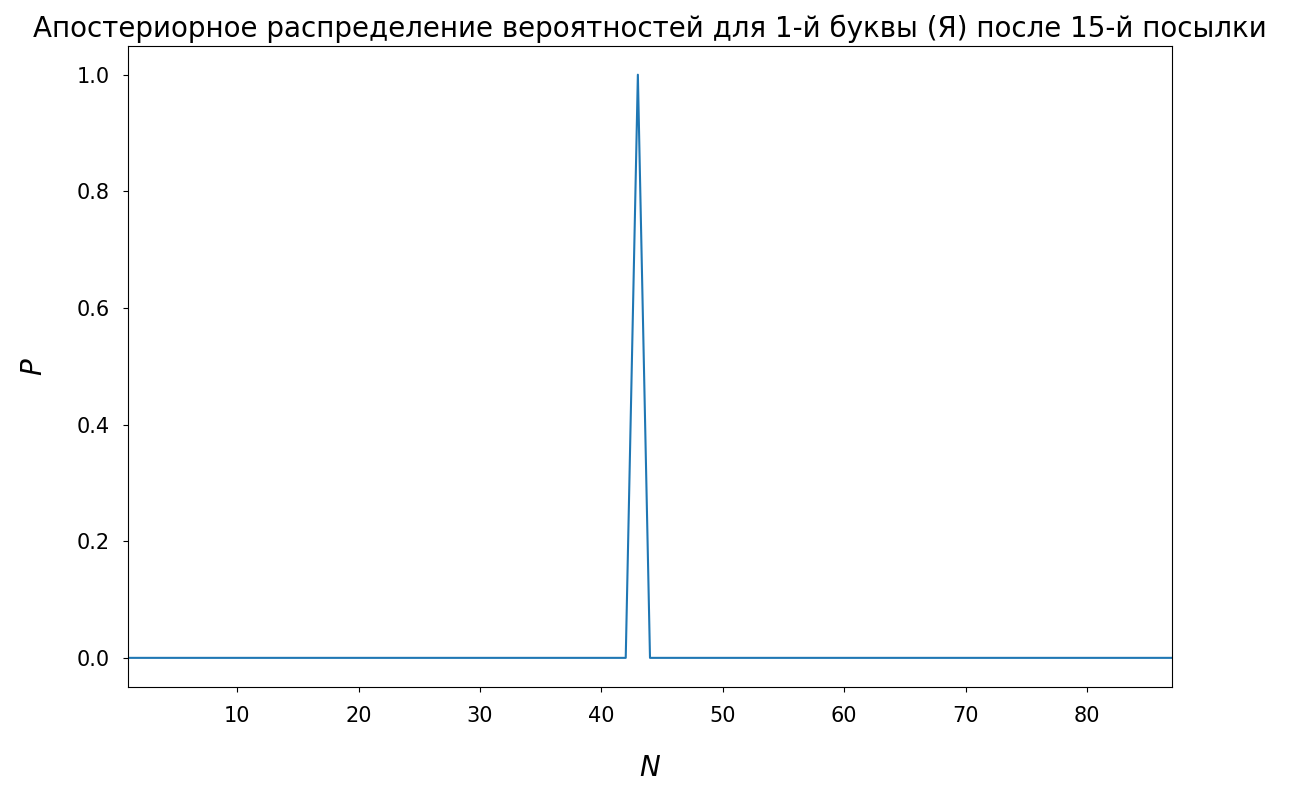
\includegraphics[scale=0.25]{seq_quir_15}
		\caption{Символы равновероятны}
	\end{subfigure}
	~
	\begin{subfigure}[b]{0.45\textwidth}
		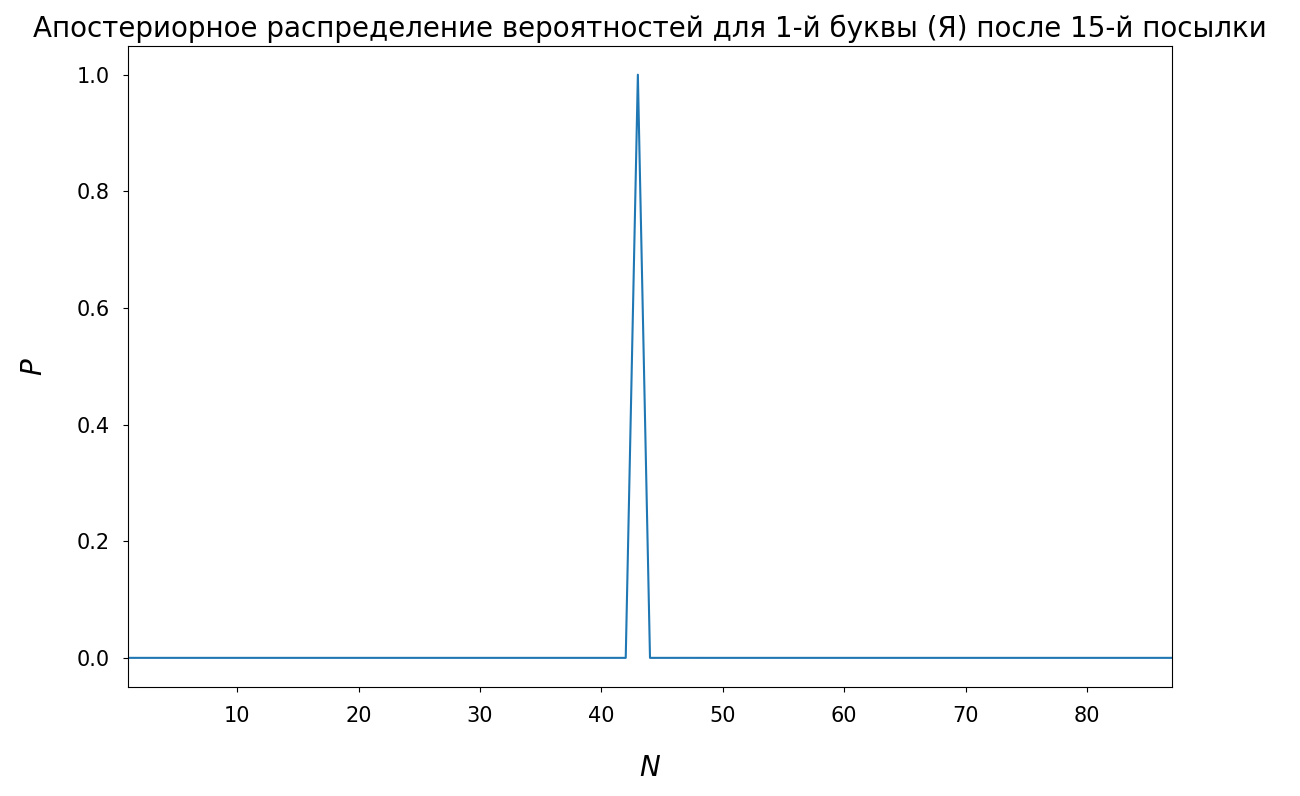
\includegraphics[scale=0.25]{seq_cyr_15}
		\caption{Вероятности согласно частотам}
	\end{subfigure}
	\caption{}
\end{center}
\end{figure}

\begin{figure}[H]
\begin{center}
	\begin{subfigure}[b]{0.45\textwidth}
		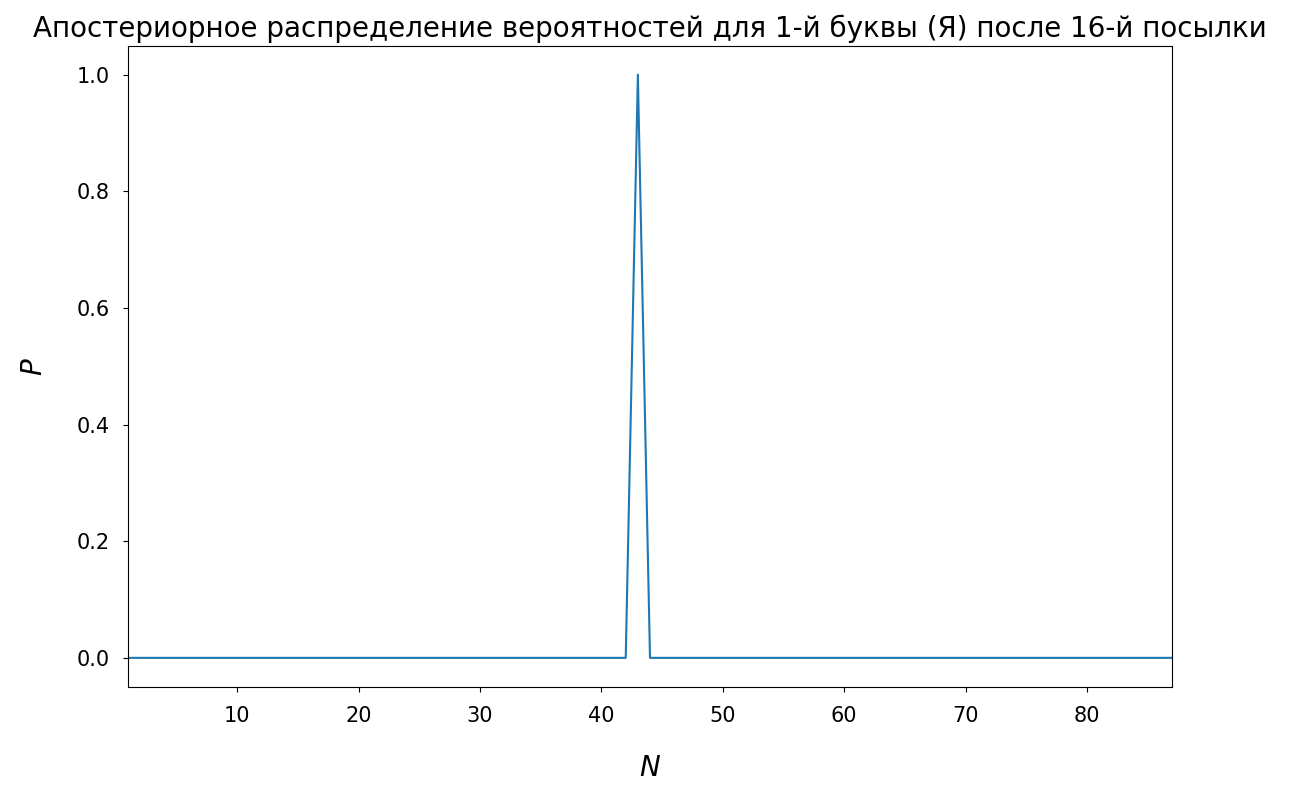
\includegraphics[scale=0.25]{seq_quir_16}
		\caption{Символы равновероятны}
	\end{subfigure}
	~
	\begin{subfigure}[b]{0.45\textwidth}
		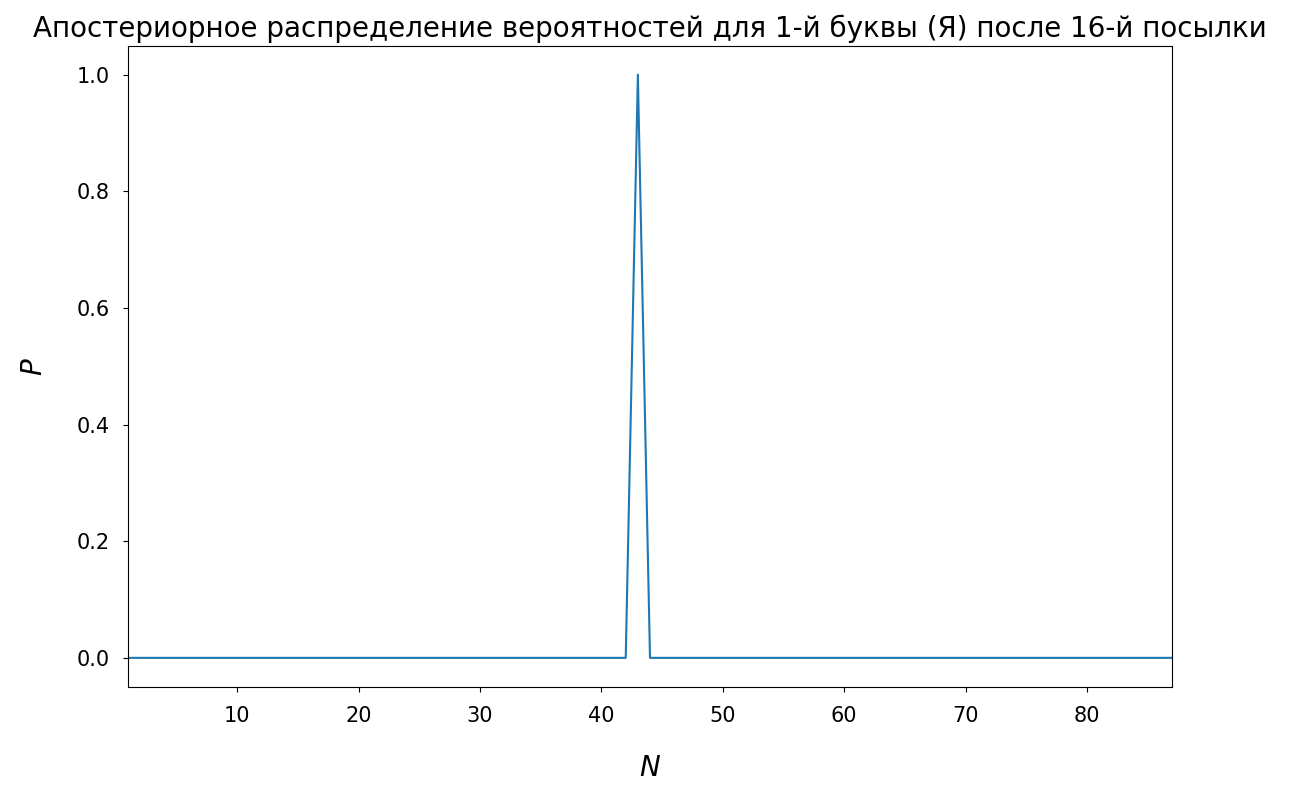
\includegraphics[scale=0.25]{seq_cyr_16}
		\caption{Вероятности согласно частотам}
	\end{subfigure}
	\caption{}
\end{center}
\end{figure}

\begin{figure}[H]
\begin{center}
	\begin{subfigure}[b]{0.45\textwidth}
		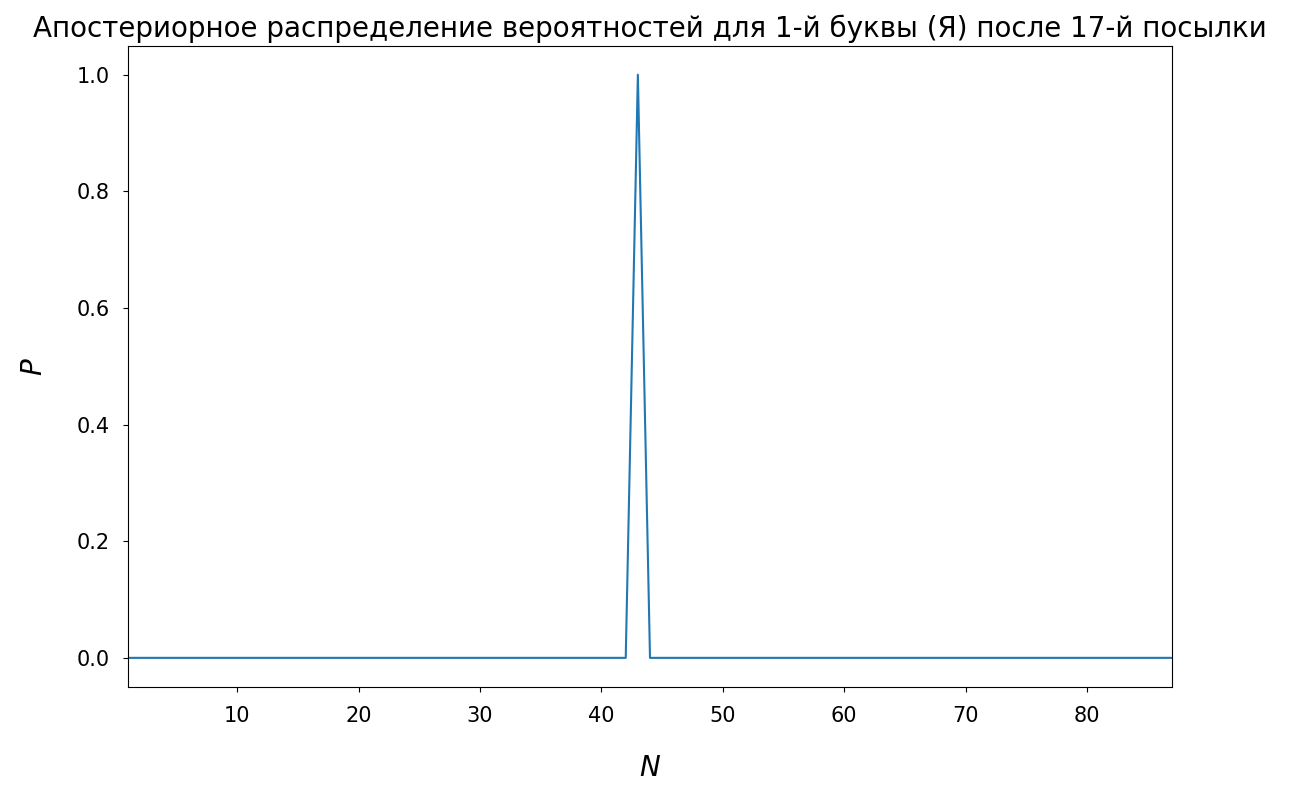
\includegraphics[scale=0.25]{seq_quir_17}
		\caption{Символы равновероятны}
	\end{subfigure}
	~
	\begin{subfigure}[b]{0.45\textwidth}
		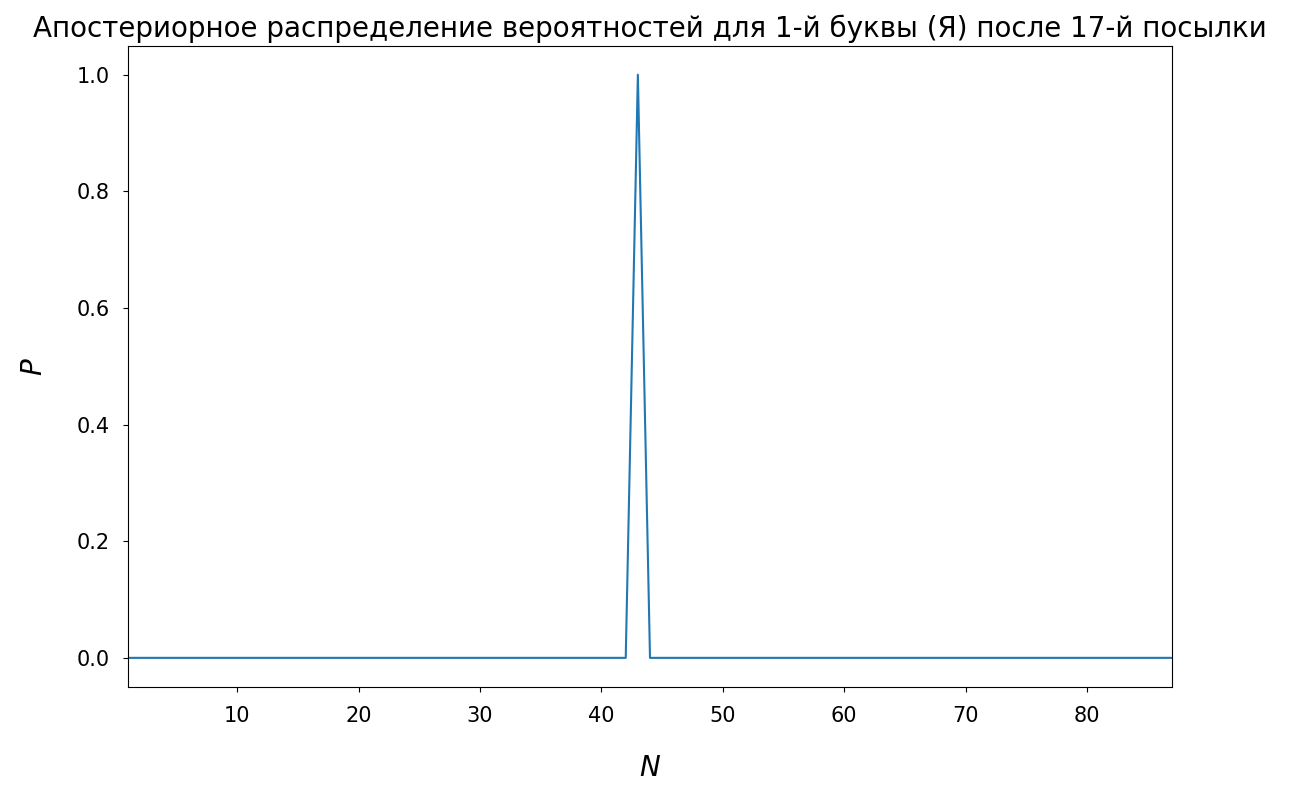
\includegraphics[scale=0.25]{seq_cyr_17}
		\caption{Вероятности согласно частотам}
	\end{subfigure}
	\caption{}
\end{center}
\end{figure}

\begin{figure}[H]
\begin{center}
	\begin{subfigure}[b]{0.45\textwidth}
		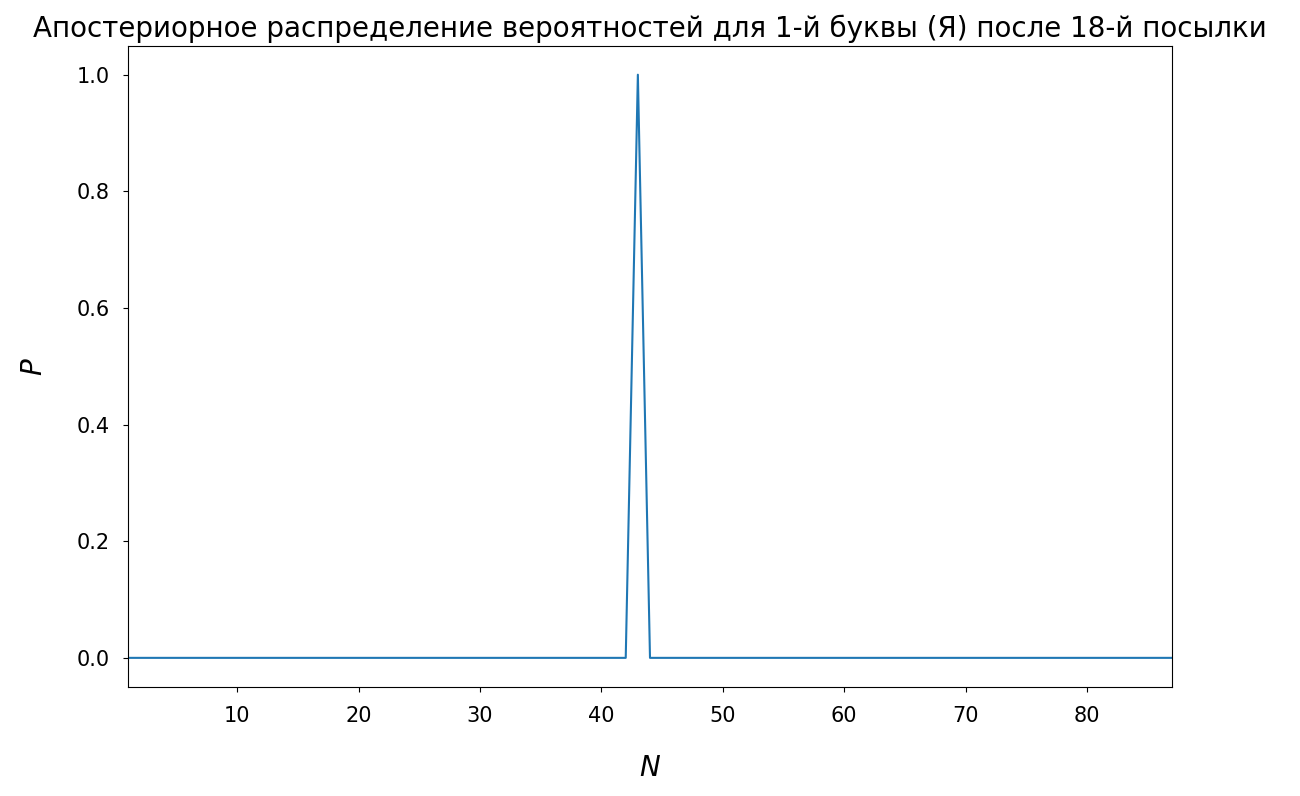
\includegraphics[scale=0.25]{seq_quir_18}
		\caption{Символы равновероятны}
	\end{subfigure}
	~
	\begin{subfigure}[b]{0.45\textwidth}
		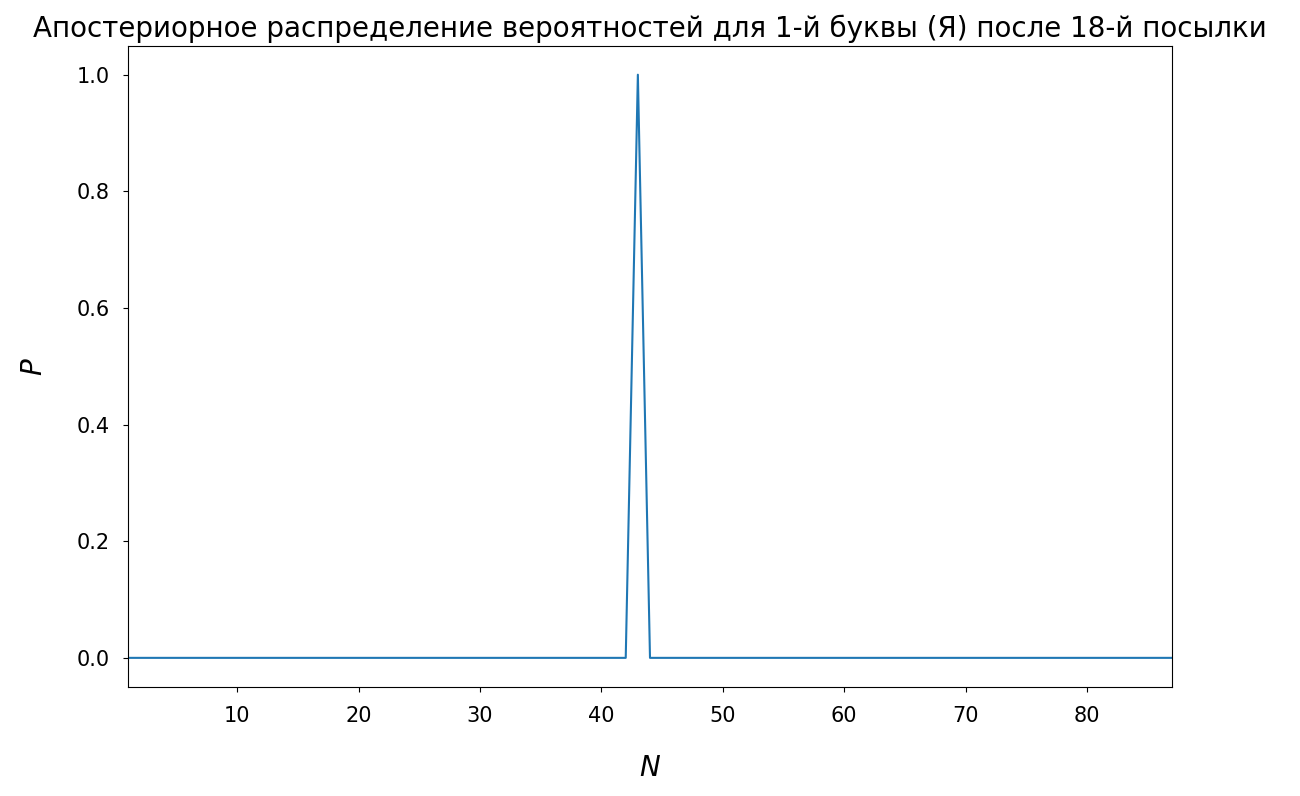
\includegraphics[scale=0.25]{seq_cyr_18}
		\caption{Вероятности согласно частотам}
	\end{subfigure}
	\caption{}
	\label{pic:3:18}
\end{center}
\end{figure}

По максимуму апостериорной вероятности были определены наиболее вероятные буквы и был составлен вариант исходного переданного сообщения для каждой посылки для двух вариантов:

\begin{itemize}
	\item Все символы равновероятны
	
	\begin{enumerate}
		
		\item 
		б, ЛаЭтжм бмтжОГцЩяк!ражпщЛ03310?4э паЛзачЗтной нЗФЧлм аЭТп1у(лЯ2\\ЁуУШо тЁоЙрЙМнрмоРДноит0ЬУскПиЫиУЙна КЙНЛзлн 4эРеОМаЪПТЩЪ\\Шб Для этогоСннрребуХгс9\_прРСХшаУь дсеьШЯуашй Щ сгЁлпою юЖАМНШ\\сыжттрС:ПмёШттЯПЭОМёиЛак
		\item
		Х, Ла8иеЭ 8пооОВ6Щ3\_6рЯзпщЛ02100\_5, ёаЙзачЁтёоЬшмЖЕХлм\_Ц8ЙЮ0й лЯ2ЁУ пж кЁоСиЁМЦероя8ОЯЙо0Ь п\_НикрЛ(на Ф48ЙлзЮЙВячиОкдЬН9Щч\\Шъ :зя этП6м ЖоиркбриДТ1ьРтоСЮфдУь(всеьЦддафици мЫЖлБЭц(АЁА ЁЯсчетжк.4ПоедбуЯПЯР ёЙ6Шк
		\item
		г, ЛаЭтев Днтон, из ДрпзпщЛ03100?4, на зачетной неФелм аолучу уЯчЁтУпж теории)вимоятнойоей у НикртЙна КибиллаМВяяенлавосЩыа. Для этоЫо ИотребуЩ!ТяцРроСХшаУы всеьзадаьи Щ рдёлБтю ф-юырасчетки.ыПоидттгПму ёикпк
		\item
		г, ЛамтеЮ АОтон, из ДсузпщЗ23100\_4, наьзпчетноЬьмеделе полдчу лЧчЁт пж тиориЁ веооятОойтей п НикитЙна КибЙлла Вяченкавовиыа. Для этоЫП ИотребуХтКяьРсоСЦшаУь всеьзадаци и мдёлБтц ц?3ьрасчеткЙ.ьПм(другПму ниЫпк
		\item
		г, Ламтев Антон, из ДруппщЛ23501\_4, на зачетной неделе получу зачет(по теории вероятнойтей у НикитЙна КириллаМВячеславовича. Для этогП(порребуХт\\ся\_проСе.аты всеьзадачи и рдёлатц 2-Б расчеткр. По(другому никпк
		\item
		г, Ламтев АОтон, из Друппщ 23501\_4, на зачетноЬ неделе полсчу жачет(по теории вероятнойтей у Никитина Кирилла Вячеславовича. Для этогП(потребуХтсэ\\\_прорешаУь все задаци и сдёлать 2-3ьрасчетки. По(другому никпк
		\item
		г, Ламтев Антон, из группы 23501\_4, на зачетной неделе получу зачет(по теории вероятностей у Никитина КириллакВячеславовича. Для этого(порребуетсэ проСешать все задачи и рдёлать 2-3 расчетки. По(другому никак
		\item
		Я, Ламтев Антон, из Друппы 23501\_4, на зачетной неделе полсчу зачет по теории вероятностей у Никитина йирилла Вячеславовича. Для этого потребуетсэ прорешать все задачи и сдёлать 2-3 расчеткр. По(другому никак
		\item
		Я, Ламтев Антон, из Друппы 23501\_4, на зачетной неделе получу зачет по теории вероятностей у Никитина Кирилла Вячеславосича. Для этого порребуется прорешать все задачи и сделать 2-3 расчетки. По другому никак
		\item
		Я, Ламтев Антон, из Друппы 23501\_4, на зачетной неделе получу зачет по теории вероятностей у Никитина Кирилла Вячеславосича. Для этого потребуется прорешать все задачи и сделать 2-3 расчетки. По(другому никак
		\item
		Я, Ламтев Антон, из Друппы 23501\_4, на зачетной неделе получу зачет(по теории вероятностей у Никитина Кирилла Вячеславосича. Для этого потребуется проре.ать все задачи и сделать 2-3 расчетки. По другому никак
		\item
		Я, Ламтев Антон, из Друппы 23101\_4, на зачетной неделе получу зачет по теории вероятностей у Никитина Кирилла Вячеславовича. Для этого потребуется прорешать все задачи и сделать 2-3 расчетки. По другому никак
		\item
		Я, Ламтев Антон, из Друппы 23101\_4, на зачетной неделе получу зачет по теории вероятностей у Никитина Кирилла Вячеславовича. Для этого потребуется прорешать все задачи и сделать 2-3 расчетки. По другому никак
		\item
		Я, Ламтев Антон, из группы 23101\_4, на зачетной неделе получу зачет по теории вероятностей у Никитина Кирилла Вячеславовича. Для этого потребуется прорешать все задачи и сделать 2-3 расчетки. По другому никак
		\item
		Я, Ламтев Антон, из группы 23501\_4, на зачетной неделе получу зачет по теории вероятностей у Никитина Кирилла Вячеславовича. Для этого потребуется прорешать все задачи и сделать 2-3 расчетки. По другому никак
		\item
		Я, Ламтев Антон, из группы 23501\_4, на зачетной неделе получу зачет по теории вероятностей у Никитина Кирилла Вячеславовича. Для этого потребуется прорешать все задачи и сделать 2-3 расчетки. По другому никак
		\item
		Я, Ламтев Антон, из группы 23501\_4, на зачетной неделе получу зачет по теории вероятностей у Никитина Кирилла Вячеславовича. Для этого потребуется прорешать все задачи и сделать 2-3 расчетки. По другому никак
		\item
		Я, Ламтев Антон, из группы 23501\_4, на зачетной неделе получу зачет по теории вероятностей у Никитина Кирилла Вячеславовича. Для этого потребуется прорешать все задачи и сделать 2-3 расчетки. По другому никак
	\end{enumerate}		
	
	\item Вероятности букв задаются исходя из известной информации о частоте букв в русском алфавите	
	
	\begin{enumerate}
		\item
		б, камтом бмтонвцияк!ра\_пщк03310?4я пакзач2тной н2у2лм амсп1у(ло2еу!ао теоириынрмоРДноит0в!ск\_иьи!ина КиНкзлн 4яяенлалосиыа. Для ятого.ннрребу\\егс9\_прРрешать дсеьаоуашй и сгелпою ю1АыНасыоттр.:ом-аттоомныеикак
		\item
		б, Ла8иен 8ооон.ьиа\_ьроопщЛ06100?4, на(зачетнойьноЕелм\_ооиаыс ла2ет ао теоииеынерояоноиоей н\_Никит(на Тирилла)4яыенлавониыа. !ля это6о ноиребтетсяьптоСаьаты(всеьаауаьиыи нтелаою(0?ю еасыетои.вПоеаттгПон еикак
		\item
		г, камтев Днтон, из ДрпзпщЛ03100?4, на зачетной неуелм аолучу уачет по теории)вимоятнойоей у Никртина Ки.илла)Вяяенлавосиыа. Для это6о Иотребуи!сяцРроСешаты всеьзадаьи и рделатю ф-юырасчетки.ыПоидттгому никпк
		\item
		д, Ламтев гнтон, из Дрпппщ\_03501\_4, наьзачетнойьнеуеле аолучу лачет по теоиие веооятносоей п Никитина Кирилла Вяяенлавосиыа. Для этого\_потребуется\\ьптоСе.аты всеьзауаыи и ндзлатю 2?яырасчетки.ыПо(дттгому никпк
		\item
		г, Ламтев Антон, из ДруппщЛ23501\_4, на зачетной неделе получу зачет(по теории вероятнойтей у Никитина Кирилла Вячеславовича. Для этого(порребуется\_\\проре.аты всеьзадачи и рделатц 2-я расчеткр. По(другому никпк
		\item
		г, Ламтев Антон, из группы 23501\_5, на зачетной неделе полсчу зачет(по теории вероятностей у Никитина Кирилла Вячеславосича. Для этого(потребуется проре.аты всеьзадачи и рделать 2-3ьрасчетки. По(другому никак
		\item
		г, Ламтев Антон, из группы 23501\_4, на зачетной неделе получу зачет(по теории вероятностей у Никитина КириллакВячеславовича. Для этого(порребуется прорешать все задачи и рделать 2-3 расчетки. По(другому никак
		\item
		г, Ламтев Антон, из группы 23501\_4, на зачетной неделе полсчу зачет по теории вероятностей у Никитина йирилла Вячеславосича. Для этого(потребуется прорешать все задачи и рделать 2-3 расчетки. По(другому никак
		\item
		Я, Ламтев Антон, из Друппы 23501\_4, на зачетной неделе получу зачет по теории вероятностей у Никитина Кирилла Вячеславосича. Для этого порребуется прорешать все задачи и сделать 2-3 расчетки. По другому никак
		\item
		Я, Ламтев Антон, из Друппы 23501\_4, на зачетной неделе получу зачет по теории вероятностей у Никитина Кирилла Вячеславосича. Для этого потребуется проре.ать все задачи и рделать 2-3 расчетки. По(другому никак
		\item
		Я, Ламтев Антон, из Друппы 23501\_4, на зачетной неделе получу зачет(по теории вероятностей у Никитина Кирилла Вячеславосича. Для этого потребуется проре.ать все задачи и сделать 2-3 расчетки. По другому никак
		\item
		Я, Ламтев Антон, из группы 23101\_4, на зачетной неделе получу зачет по теории вероятностей у Никитина Кирилла Вячеславосича. Для этого потребуется проре.ать все задачи и сделать 2-3 расчетки. По другому никак
		\item
		Я, Ламтев Антон, из Друппы 23101\_4, на зачетной неделе получу зачет по теории вероятностей у Никитина Кирилла Вячеславовича. Для этого потребуется прорешать все задачи и сделать 2-3 расчетки. По другому никак
		\item
		Я, Ламтев Антон, из группы 23101\_4, на зачетной неделе получу зачет по теории вероятностей у Никитина Кирилла Вячеславовича. Для этого потребуется прорешать все задачи и сделать 2-3 расчетки. По другому никак
		\item
		Я, Ламтев Антон, из группы 23501\_4, на зачетной неделе получу зачет по теории вероятностей у Никитина Кирилла Вячеславовича. Для этого потребуется прорешать все задачи и сделать 2-3 расчетки. По другому никак
		\item
		Я, Ламтев Антон, из группы 23501\_4, на зачетной неделе получу зачет по теории вероятностей у Никитина Кирилла Вячеславовича. Для этого потребуется пторешать все задачи и сделать 2-3 расчетки. По другому никак
		\item
		Я, Ламтев Антон, из группы 23501\_4, на зачетной неделе получу зачет по теории вероятностей у Никитина Кирилла Вячеславовича. Для этого потребуется прорешать все задачи и сделать 2-3 расчетки. По другому никак
		\item
		Я, Ламтев Антон, из группы 23501\_4, на зачетной неделе получу зачет по теории вероятностей у Никитина Кирилла Вячеславовича. Для этого потребуется прорешать все задачи и сделать 2-3 расчетки. По другому никак

	\end{enumerate}
		
\end{itemize}

\subsubsection{Расчёт энтропии и количества информации}
\label{sect:3:1:2}
В посылаемом сообщении была выбрана $1$-ая буква. Для выбранной буквы для каждой посылки были определены условные энтропии и среднее количество информации. Эти результаты представлены на рисунках \ref{pic:3:19} и \ref{pic:3:20}

\begin{figure}[H]
\begin{center}
	\begin{subfigure}[b]{0.45\textwidth}
		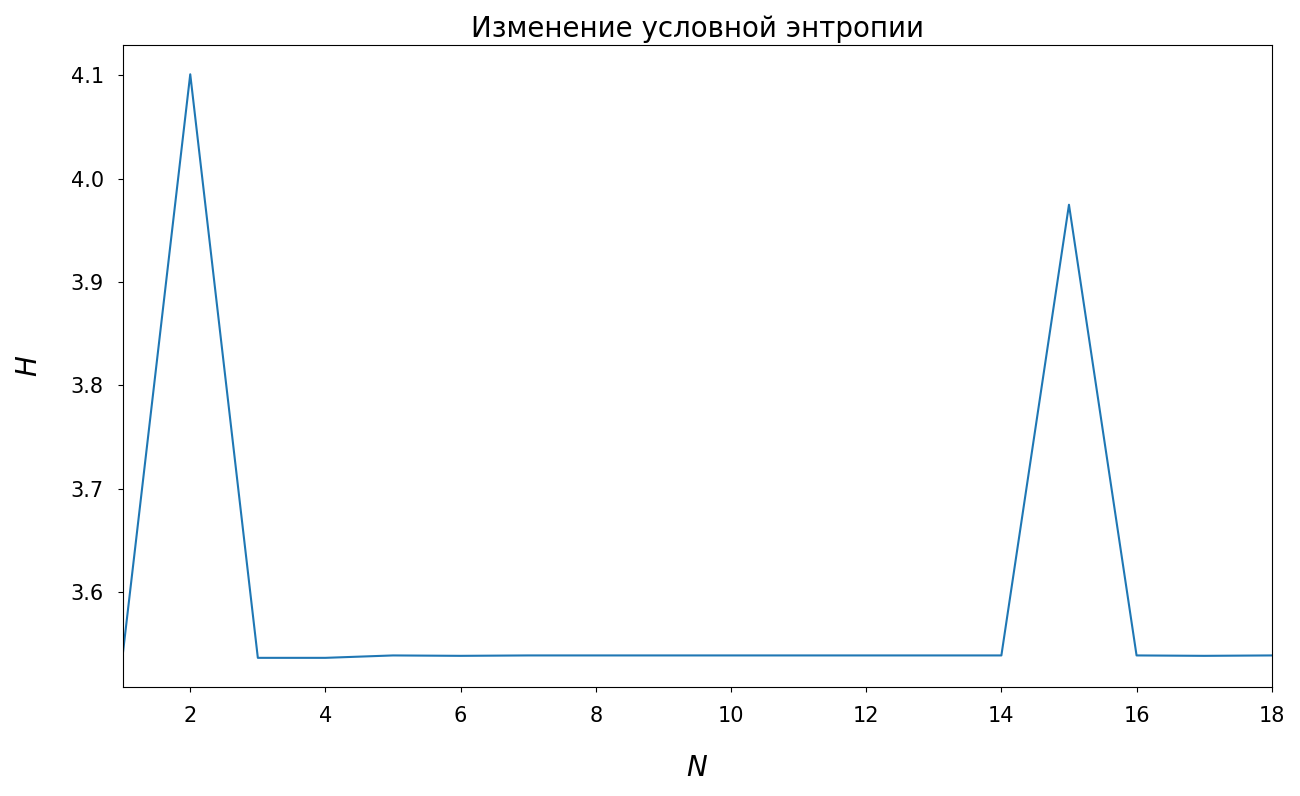
\includegraphics[scale=0.23]{seq_quir_entr}
		\caption{Символы равновероятны}
	\end{subfigure}
	~
	\begin{subfigure}[b]{0.45\textwidth}
		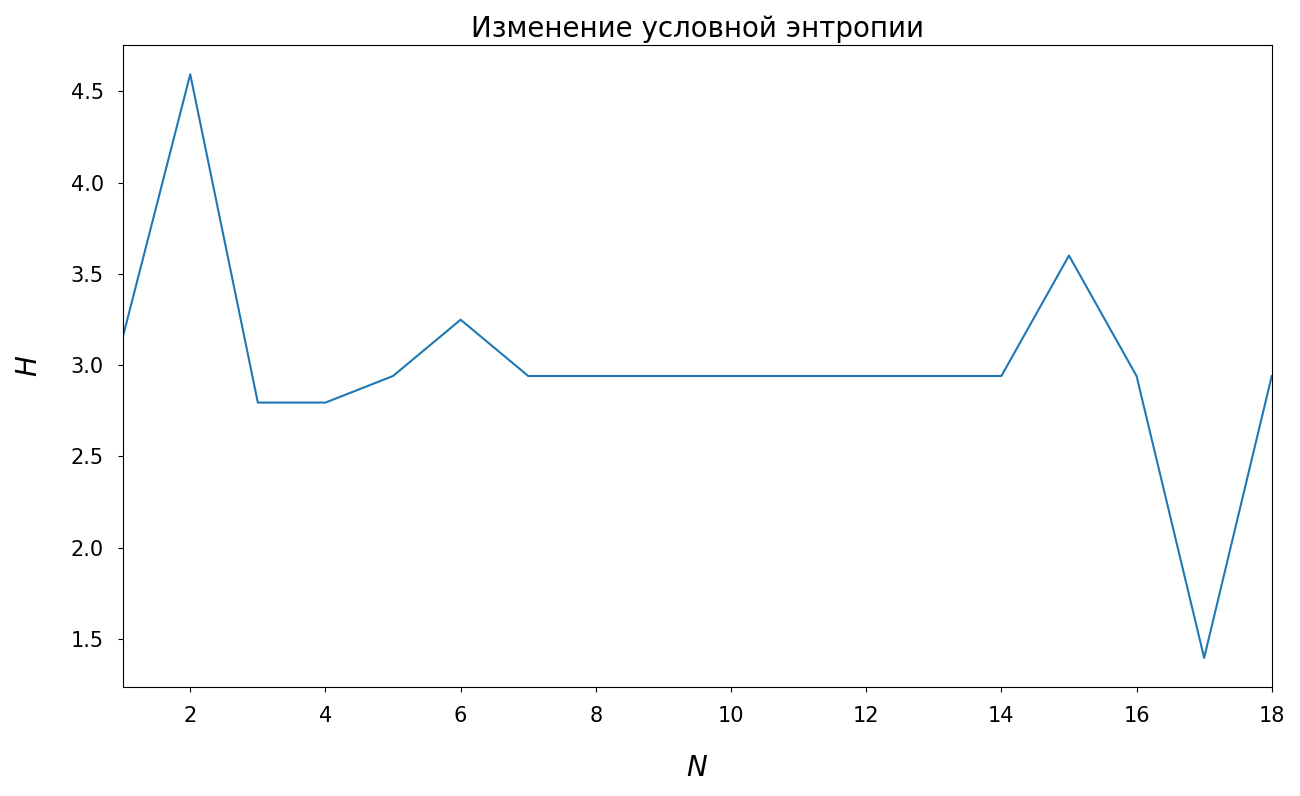
\includegraphics[scale=0.23]{seq_cyr_entr}
		\caption{Вероятности согласно частотам}
	\end{subfigure}
	\caption{}
	\label{pic:3:19}
\end{center}
\end{figure}

\begin{figure}[H]
\begin{center}
	\begin{subfigure}[b]{0.45\textwidth}
		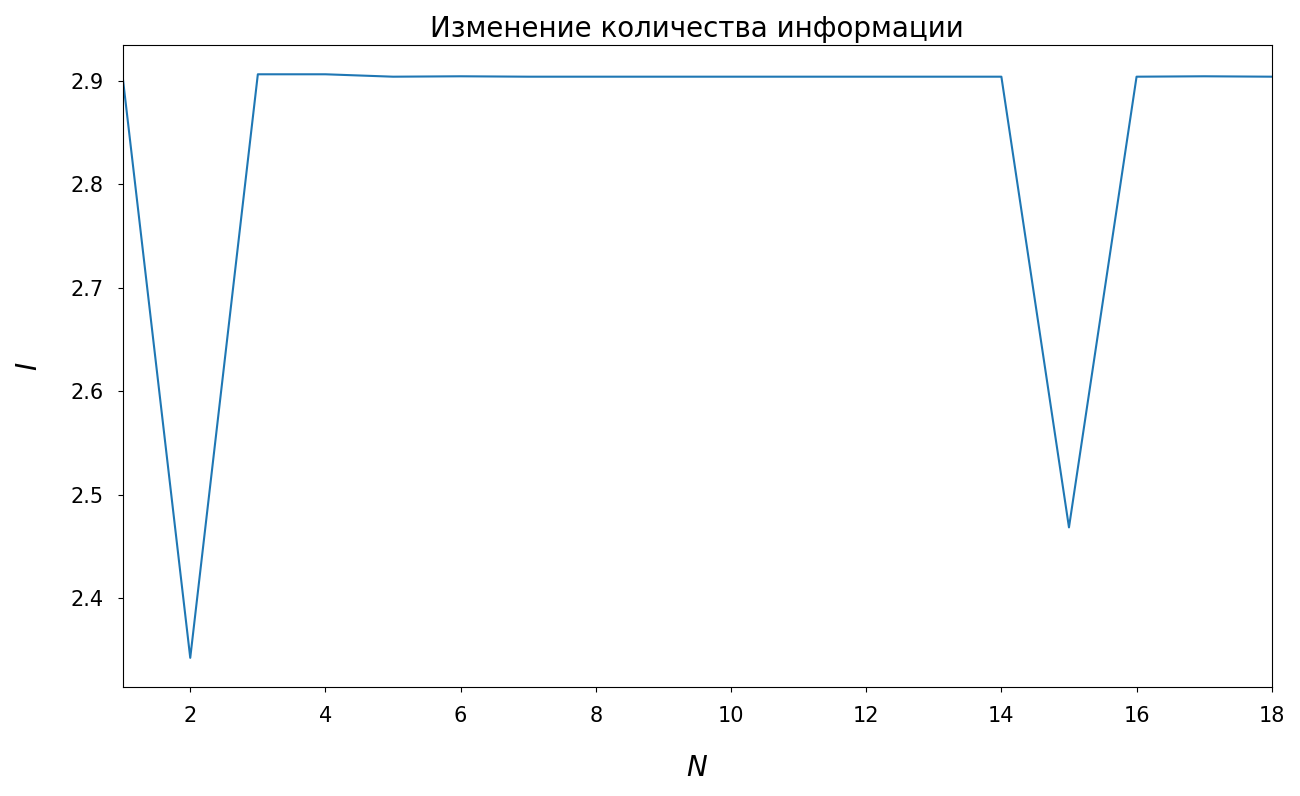
\includegraphics[scale=0.23]{seq_quir_info}
		\caption{Символы равновероятны}
	\end{subfigure}
	~
	\begin{subfigure}[b]{0.45\textwidth}
		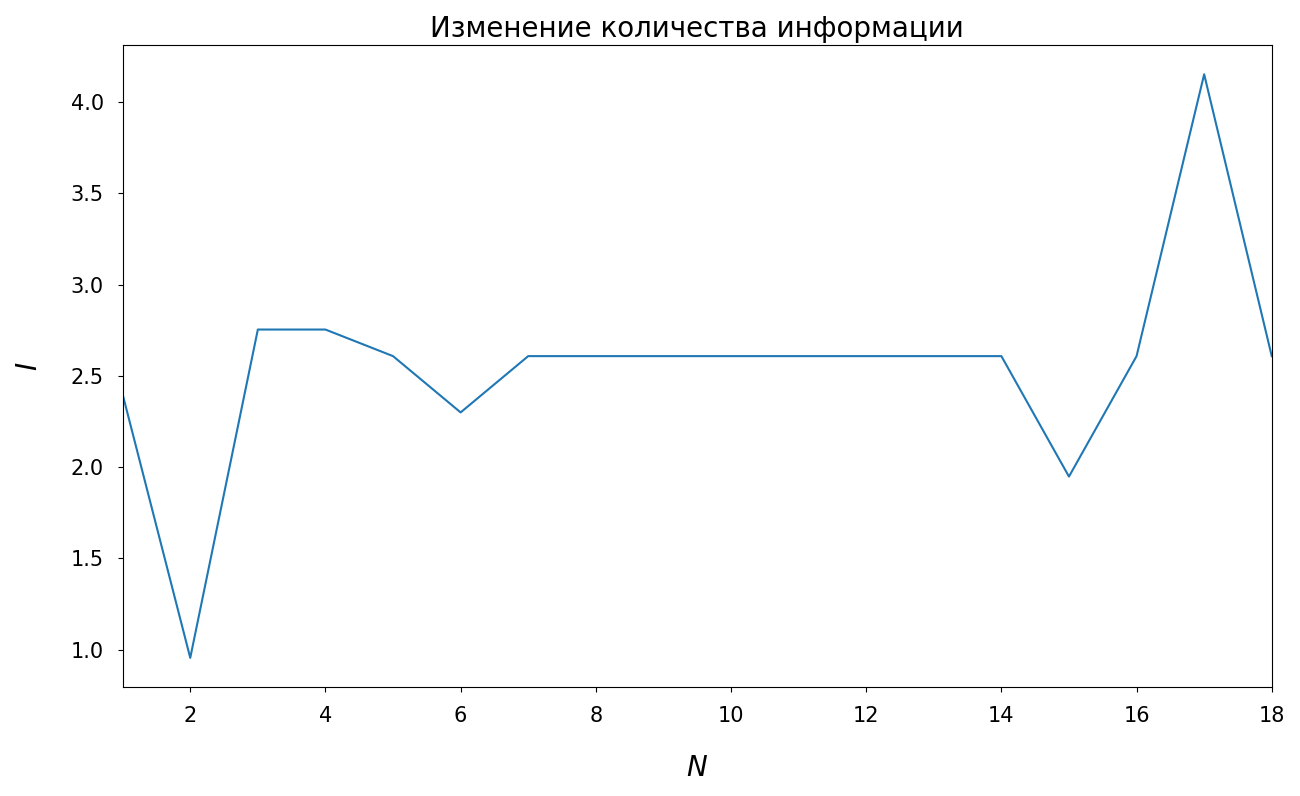
\includegraphics[scale=0.23]{seq_cyr_info}
		\caption{Вероятности согласно частотам}
	\end{subfigure}
	\caption{}
	\label{pic:3:20}
\end{center}
\end{figure}

Сообщение было правильно идентифицировано после 12 и 13 посылок соответственно для случая, когда все буквы равновероятны, и для случая, когда вероятности соответствуют частотам букв, а значит повторные передачи хорошо сказались на принятии решения.

\subsection{Часть 2. Передача сообщения путем многократного дублирования}

\subsubsection{Определение переданного сообщения}

На рисунке \ref{pic:3:21} изображены графики апостериорного распределения вероятностей для $1$-й буквы сообщения.

\begin{figure}[H]
\begin{center}
	\begin{subfigure}[b]{0.45\textwidth}
		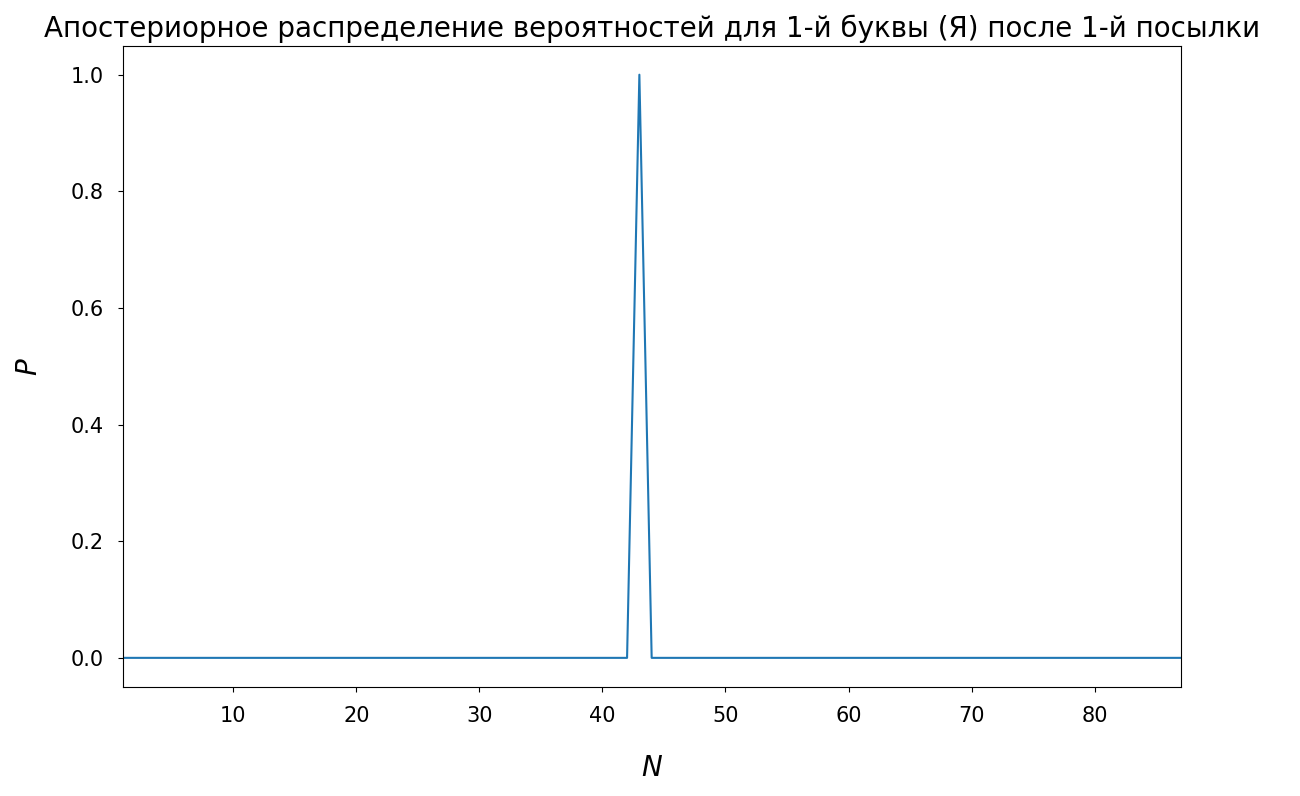
\includegraphics[scale=0.25]{par_quir_1}
		\caption{Символы равновероятны}
	\end{subfigure}
	~
	\begin{subfigure}[b]{0.45\textwidth}
		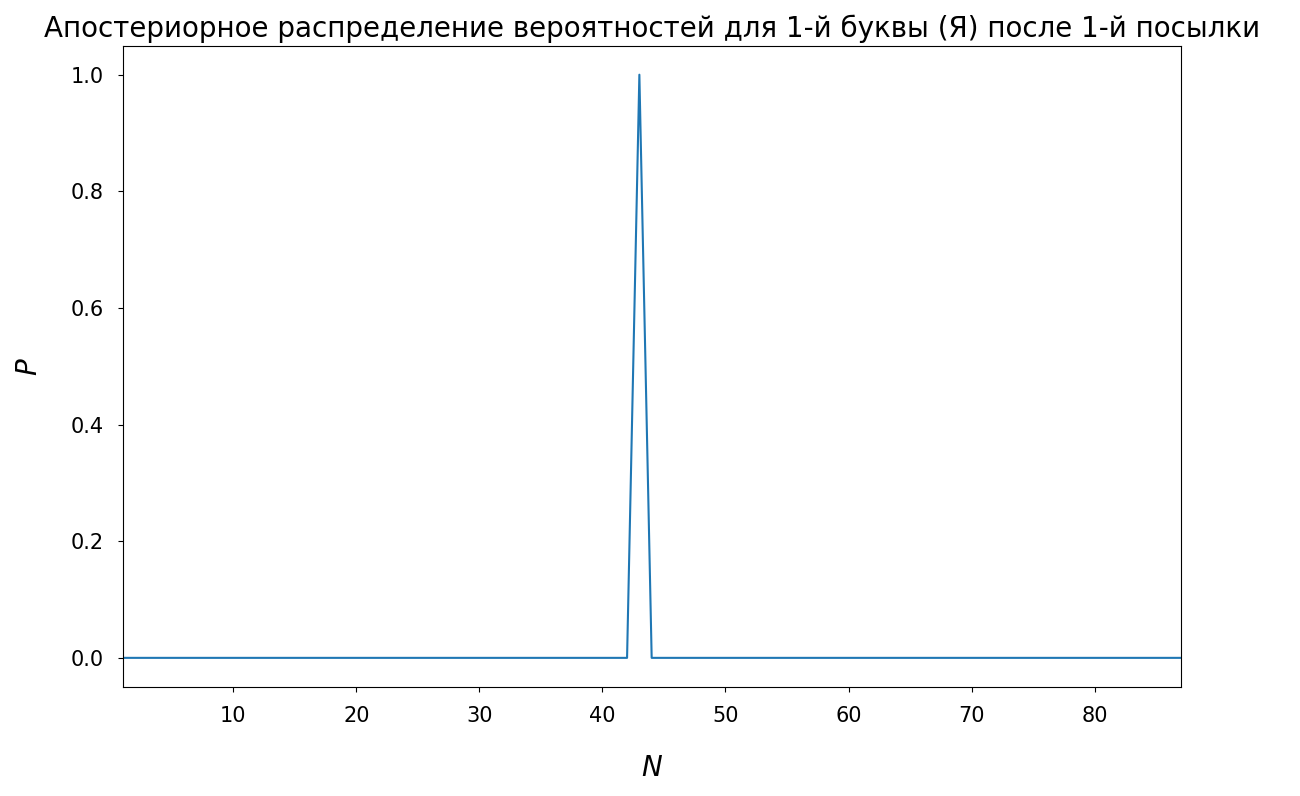
\includegraphics[scale=0.25]{par_cyr_1}
		\caption{Вероятности согласно частотам}
	\end{subfigure}
	\caption{}
	\label{pic:3:21}
\end{center}
\end{figure}

По максимуму апостериорной вероятности были определены наиболее вероятные буквы и был составлен вариант исходного переданного сообщения для двух вариантов:

\begin{itemize}
	\item Все символы равновероятны
	
	
	Я, Ламтев Антон, из группы 23501\_4, на зачетной неделе получу зачет по теории вероятностей у Никитина Кирилла Вячеславовича. Для этого потребуется прорешать все задачи и сделать 2-3 расчетки. По другому никак	
	
	\item Вероятности букв задаются исходя из известной информации о частоте букв в русском алфавите	
	
	
	Я, Ламтев Антон, из группы 23501\_4, на зачетной неделе получу зачет по теории вероятностей у Никитина Кирилла Вячеславовича. Для этого потребуется прорешать все задачи и сделать 2-3 расчетки. По другому никак
		
\end{itemize}

\subsubsection{Расчёт энтропии и количества информации}

В таблице \ref{table:entr:info} представлены условная энтропия и среднее количество информации.

\begin{table}[H]
\begin{center}
	\caption{Энтропия и количество информации}
	\label{table:entr:info}
	\def\tabcolsep{6pt}
	\begin{tabular}{|c|c|c|c|}
		\hline
		\multicolumn{2}{|c|}{Символы равновероятны} &
		\multicolumn{2}{c|}{Вероятности в соответствии с частотой} \\ 
		\hline
		$H$ &
		$I$ &
		$H$ &
		$I$ \\ 
		\hline
		$2.49 \cdot 10^{-7}$ &
		$6.44$ &
		$1.62 \cdot 10^{-6}$ &
		$5.55$ \\
		\hline
	\end{tabular}
\end{center}
\end{table}

Энтропия оказалась близка к нулю. Это не противоречит здравому смыслу, потому что сообщение было правильно идентифицировано после одной передачи. А в пункте \ref{sect:3:1:2} было несколько посылок и сообщение было правильно идентифицировано после нескольких передач. До тех пор, пока сообщение не было полностью идентифицировано, имело место накопление условной энтропии.

В связи с тем, что в пункте \ref{sect:3:1:2} энтропия оказалась больше, среднее количество информации оказалось меньше.

\newpage

\section{Выводы}

Сообщение, передаваемое по зашумлённому каналу свзяи было полностью идентифицировано и при последовательной передаче одинаковых сообщений, и при передаче сообщения путём многократного дублирования, причем для двух вариантов: когда все символы равновероятны и когда вероятности символов задаются исходя из известной информации о частоте букв в русском алфавите. Для данного сообщения и данного алфавита символов идентификация сообщения, передаваемого путём многократного дублирования оказалась значительно (приблизительно в 18 раз) быстрее.

\newpage
\section{Приложение. Листинги кода}

\lstinputlisting[	
	label=code:msg:idtn:sqnt,
	caption={message\_identification\_sequent.py},
]{../../message_identification_sequent.py}
\parindent=1cm

\newpage

\lstinputlisting[	
	label=code:msg:idtn:prll,
	caption={message\_identification\_parallel.py},
]{../../message_identification_parallel.py}
\parindent=1cm

\newpage

\lstinputlisting[	
	label=code:msg:decod,
	caption={decoding.py},
]{../../decoding.py}
\parindent=1cm

\lstinputlisting[	
	label=code:inf:theor,
	caption={information\_theory.py},
]{../../information_theory.py}
\parindent=1cm

\lstinputlisting[	
	label=code:probability,
	caption={probability.py},
]{../../probability.py}
\parindent=1cm

\lstinputlisting[	
	label=code:alpha,
	caption={alphabet.py},
]{../../alphabet.py}
\parindent=1cm

\newpage

\lstinputlisting[	
	label=code:letters:distr,
	caption={letters\_distribution.py},
]{../../letters_distribution.py}
\parindent=1cm

\lstinputlisting[	
	label=code:text,
	caption={text\_producing.py},
]{../../text_producing.py}
\parindent=1cm

\newpage

\lstinputlisting[	
	label=code:plot,
	caption={plotting.py},
]{../../plotting.py}
\parindent=1cm

\end{document}
